\begin{filecontents*}[overwrite]{nocompiler-references.bib}
@misc{nocompiler, author={Hideaki Takahashi}, title={{NoCompiler}: Source, proofs, design documents, and trial files at commit 998ae0d}, year={2026}, url={https://github.com/h5i-dev/NoCompiler/tree/998ae0df1d52a7d7ce0ed7bca6113d417eec2c39}, note={Pinned artifact; full revision 998ae0df1d52a7d7ce0ed7bca6113d417eec2c39}}
@inproceedings{pcc96, author={George C. Necula and Peter Lee}, title={Safe Kernel Extensions Without Run-Time Checking}, booktitle={Proceedings of the Second USENIX Symposium on Operating Systems Design and Implementation (OSDI '96)}, pages={229--243}, year={1996}, publisher={ACM}, address={New York, NY, USA}, doi={10.1145/238721.238781}}
@inproceedings{pcc97, author={George C. Necula}, title={Proof-Carrying Code}, booktitle={Proceedings of the 24th ACM SIGPLAN-SIGACT Symposium on Principles of Programming Languages (POPL '97)}, pages={106--119}, year={1997}, publisher={ACM}, address={New York, NY, USA}, doi={10.1145/263699.263712}}
@article{tal, author={Greg Morrisett and David Walker and Karl Crary and Neal Glew}, title={From System {F} to Typed Assembly Language}, journal={ACM Transactions on Programming Languages and Systems}, volume={21}, number={3}, pages={527--568}, year={1999}, month=may, doi={10.1145/319301.319345}}
@inproceedings{dtal, author={Hongwei Xi and Robert Harper}, title={A Dependently Typed Assembly Language}, booktitle={Proceedings of the Sixth ACM SIGPLAN International Conference on Functional Programming (ICFP '01)}, pages={169--180}, year={2001}, publisher={ACM}, address={New York, NY, USA}, doi={10.1145/507635.507657}}
@inproceedings{aliastypes, author={Frederick Smith and David Walker and Greg Morrisett}, title={Alias Types}, booktitle={Programming Languages and Systems (ESOP 2000)}, editor={Gert Smolka}, series={Lecture Notes in Computer Science}, volume={1782}, pages={366--381}, year={2000}, publisher={Springer}, address={Berlin, Heidelberg}, doi={10.1007/3-540-46425-5_24}}
@techreport{ltal, author={James Cheney and Greg Morrisett}, title={A Linearly Typed Assembly Language}, institution={Cornell University}, number={TR2003-1900}, year={2003}, month=jun, url={https://hdl.handle.net/1813/5613}}
@inproceedings{liquid, author={Patrick M. Rondon and Ming Kawaguchi and Ranjit Jhala}, title={Liquid Types}, booktitle={Proceedings of the 29th ACM SIGPLAN Conference on Programming Language Design and Implementation (PLDI '08)}, pages={159--169}, year={2008}, publisher={ACM}, address={New York, NY, USA}, doi={10.1145/1375581.1375602}}
@inproceedings{llliquid, author={Patrick Maxim Rondon and Ming Kawaguchi and Ranjit Jhala}, title={Low-Level Liquid Types}, booktitle={Proceedings of the 37th Annual ACM SIGPLAN-SIGACT Symposium on Principles of Programming Languages (POPL '10)}, pages={131--144}, year={2010}, publisher={ACM}, address={New York, NY, USA}, doi={10.1145/1706299.1706316}}
@inproceedings{sfi, author={Robert Wahbe and Steven Lucco and Thomas E. Anderson and Susan L. Graham}, title={Efficient Software-Based Fault Isolation}, booktitle={Proceedings of the Fourteenth ACM Symposium on Operating Systems Principles (SOSP '93)}, pages={203--216}, year={1993}, publisher={ACM}, address={New York, NY, USA}, doi={10.1145/168619.168635}}
@inproceedings{nacl, author={Bennet Yee and David Sehr and Gregory Dardyk and J. Bradley Chen and Robert Muth and Tavis Ormandy and Shiki Okasaka and Neha Narula and Nicholas Fullagar}, title={Native Client: A Sandbox for Portable, Untrusted x86 Native Code}, booktitle={2009 30th IEEE Symposium on Security and Privacy}, pages={79--93}, year={2009}, publisher={IEEE}, address={Los Alamitos, CA, USA}, doi={10.1109/SP.2009.25}}
@inproceedings{rocksalt, author={Greg Morrisett and Gang Tan and Joseph Tassarotti and Jean-Baptiste Tristan and Edward Gan}, title={RockSalt: Better, Faster, Stronger SFI for the x86}, booktitle={Proceedings of the 33rd ACM SIGPLAN Conference on Programming Language Design and Implementation (PLDI '12)}, pages={395--404}, year={2012}, publisher={ACM}, address={New York, NY, USA}, doi={10.1145/2254064.2254111}}
@inproceedings{prevail, author={Elazar Gershuni and Nadav Amit and Arie Gurfinkel and Nina Narodytska and Jorge A. Navas and Noam Rinetzky and Leonid Ryzhyk and Mooly Sagiv}, title={Simple and Precise Static Analysis of Untrusted Linux Kernel Extensions}, booktitle={Proceedings of the 40th ACM SIGPLAN Conference on Programming Language Design and Implementation (PLDI '19)}, pages={1069--1084}, year={2019}, publisher={ACM}, address={New York, NY, USA}, doi={10.1145/3314221.3314590}}
@inproceedings{seplogic, author={John C. Reynolds}, title={Separation Logic: A Logic for Shared Mutable Data Structures}, booktitle={Proceedings of the 17th Annual IEEE Symposium on Logic in Computer Science (LICS 2002)}, pages={55--74}, year={2002}, publisher={IEEE Computer Society}, address={Los Alamitos, CA, USA}, doi={10.1109/LICS.2002.1029817}}
@article{compcert, author={Xavier Leroy}, title={Formal Verification of a Realistic Compiler}, journal={Communications of the ACM}, volume={52}, number={7}, pages={107--115}, year={2009}, month=jul, doi={10.1145/1538788.1538814}}
@inproceedings{cakeml, author={Ramana Kumar and Magnus O. Myreen and Michael Norrish and Scott Owens}, title={{CakeML}: A Verified Implementation of {ML}}, booktitle={Proceedings of the 41st ACM SIGPLAN-SIGACT Symposium on Principles of Programming Languages (POPL '14)}, pages={179--191}, year={2014}, publisher={ACM}, address={New York, NY, USA}, doi={10.1145/2535838.2535841}}
@inproceedings{sel4tv, author={Thomas Arthur Leck Sewell and Magnus O. Myreen and Gerwin Klein}, title={Translation Validation for a Verified {OS} Kernel}, booktitle={Proceedings of the 34th ACM SIGPLAN Conference on Programming Language Design and Implementation (PLDI '13)}, pages={471--482}, year={2013}, publisher={ACM}, address={New York, NY, USA}, doi={10.1145/2491956.2462183}}
@inproceedings{islaris, author={Michael Sammler and Angus Hammond and Rodolphe Lepigre and Brian Campbell and Jean Pichon-Pharabod and Derek Dreyer and Deepak Garg and Peter Sewell}, title={Islaris: Verification of Machine Code Against Authoritative {ISA} Semantics}, booktitle={Proceedings of the 43rd ACM SIGPLAN International Conference on Programming Language Design and Implementation (PLDI '22)}, pages={825--840}, year={2022}, publisher={ACM}, address={New York, NY, USA}, doi={10.1145/3519939.3523434}}
@article{sail, author={Alasdair Armstrong and Thomas Bauereiss and Brian Campbell and Alastair Reid and Kathryn E. Gray and Robert M. Norton and Prashanth Mundkur and Mark Wassell and Jon French and Christopher Pulte and Shaked Flur and Ian Stark and Neel Krishnaswami and Peter Sewell}, title={{ISA} Semantics for {ARMv8-A}, {RISC-V}, and {CHERI-MIPS}}, journal={Proceedings of the ACM on Programming Languages}, volume={3}, number={POPL}, articleno={71}, numpages={31}, year={2019}, month=jan, doi={10.1145/3290384}}
@inproceedings{omega, author={William Pugh}, title={The {Omega} Test: A Fast and Practical Integer Programming Algorithm for Dependence Analysis}, booktitle={Proceedings of the 1991 ACM/IEEE Conference on Supercomputing (Supercomputing '91)}, pages={4--13}, year={1991}, publisher={ACM}, address={New York, NY, USA}, doi={10.1145/125826.125848}}
@article{rustbelt, author={Ralf Jung and Jacques-Henri Jourdan and Robbert Krebbers and Derek Dreyer}, title={{RustBelt}: Securing the Foundations of the {Rust} Programming Language}, journal={Proceedings of the ACM on Programming Languages}, volume={2}, number={POPL}, articleno={66}, numpages={34}, year={2018}, month=jan, doi={10.1145/3158154}}
@inproceedings{funtal, author={Daniel Patterson and Jamie Perconti and Christos Dimoulas and Amal Ahmed}, title={{FunTAL}: Reasonably Mixing a Functional Language with Assembly}, booktitle={Proceedings of the 38th ACM SIGPLAN Conference on Programming Language Design and Implementation (PLDI '17)}, pages={495--509}, year={2017}, publisher={ACM}, address={New York, NY, USA}, doi={10.1145/3062341.3062347}}
@inproceedings{myreen, author={Magnus O. Myreen and Michael J. C. Gordon}, title={Hoare Logic for Realistically Modelled Machine Code}, booktitle={Tools and Algorithms for the Construction and Analysis of Systems (TACAS 2007)}, editor={Orna Grumberg and Michael Huth}, series={Lecture Notes in Computer Science}, volume={4424}, pages={568--582}, year={2007}, publisher={Springer}, address={Berlin, Heidelberg}, doi={10.1007/978-3-540-71209-1_44}}
@inproceedings{refinedc, author={Michael Sammler and Rodolphe Lepigre and Robbert Krebbers and Kayvan Memarian and Derek Dreyer and Deepak Garg}, title={{RefinedC}: Automating the Foundational Verification of {C} Code with Refined Ownership Types}, booktitle={Proceedings of the 42nd ACM SIGPLAN International Conference on Programming Language Design and Implementation (PLDI '21)}, pages={158--174}, year={2021}, publisher={ACM}, address={New York, NY, USA}, doi={10.1145/3453483.3454036}}
@article{cn, author={Christopher Pulte and Dhruv C. Makwana and Thomas Sewell and Kayvan Memarian and Peter Sewell and Neel Krishnaswami}, title={{CN}: Verifying Systems {C} Code with Separation-Logic Refinement Types}, journal={Proceedings of the ACM on Programming Languages}, volume={7}, number={POPL}, articleno={1}, numpages={32}, year={2023}, month=jan, doi={10.1145/3571194}}
@manual{riscvspec, author={{RISC-V International}}, title={The {RISC-V} Instruction Set Manual, Volume {I}: Unprivileged Architecture}, organization={RISC-V International}, note={Ratified version 20260120}, year={2026}, month=jan, url={https://docs.riscv.org/reference/isa/v20260120/unpriv/unpriv-index.html}}
@misc{musl, author={Rich Felker and others}, title={musl libc, release 1.2.5}, year={2024}, month=feb, url={https://musl.libc.org/}, note={Released February 29, 2024; accessed November 23, 2026}}
@misc{sailriscv, author={{RISC-V International}}, title={Sail {RISC-V} Model}, year={2026}, url={https://github.com/riscv/sail-riscv}, note={Formal specification of the RISC-V architecture in Sail; accessed November 23, 2026}}
@inproceedings{lean, author={Leonardo de Moura and Sebastian Ullrich}, title={The {Lean} 4 Theorem Prover and Programming Language}, booktitle={Automated Deduction -- CADE 28}, editor={Andr{\'e} Platzer and Geoff Sutcliffe}, series={Lecture Notes in Computer Science}, volume={12699}, pages={625--635}, year={2021}, publisher={Springer}, address={Cham}, doi={10.1007/978-3-030-79876-5_37}}
@inproceedings{ownptr, author={Izumi Tanaka and Ken Sakayori and Naoki Kobayashi}, title={Ownership Types for Verification of Programs with Pointer Arithmetic}, booktitle={Proceedings of the 2024 ACM SIGPLAN International Workshop on Partial Evaluation and Program Manipulation (PEPM '24)}, pages={94--106}, year={2024}, publisher={ACM}, address={New York, NY, USA}, doi={10.1145/3635800.3636965}}
@inproceedings{ebpfrange, author={Harishankar Vishwanathan and Matan Shachnai and Srinivas Narayana and Santosh Nagarakatte}, title={Verifying the Verifier: {eBPF} Range Analysis Verification}, booktitle={Computer Aided Verification (CAV 2023), Part III}, editor={Constantin Enea and Akash Lal}, series={Lecture Notes in Computer Science}, volume={13966}, pages={226--251}, year={2023}, publisher={Springer}, address={Cham}, doi={10.1007/978-3-031-37709-9_12}}
\end{filecontents*}
\documentclass[sigconf,nonacm]{acmart}
\usepackage{amsmath}
\usepackage{booktabs}
\usepackage{enumitem}
\usepackage{alltt}
\usepackage{mathpartir}
\setlist[itemize]{leftmargin=1.2em,labelsep=0.4em,itemsep=1pt,parsep=0pt,topsep=2pt}
\usepackage{tikz}
\usetikzlibrary{arrows.meta,positioning}
\settopmatter{printacmref=false,printfolios=true}
\setcopyright{none}
\newcommand{\sys}{\textnormal{NoCompiler}}
\newcommand{\code}[1]{\texttt{\small #1}}
\newcommand{\lean}[1]{\textnormal{\texttt{\small #1}}}
\setlength{\emergencystretch}{2em}
\AtBeginDocument{\clubpenalty=150 \widowpenalty=150 \displaywidowpenalty=150}
\renewcommand{\figurename}{Fig.}
% notation
\newcommand{\B}{\mathbb{B}}
\newcommand{\Z}{\mathbb{Z}}
\newcommand{\N}{\mathbb{N}}
\newcommand{\W}{\mathsf{Word}}
\newcommand{\sem}[1]{[\![#1]\!]}
\newcommand{\ev}[2]{[\![#1]\!]_{#2}}
\newcommand{\inttype}[1]{\mathsf{int}(#1)}
\newcommand{\bytes}[3]{#1\mapsto\mathsf{bytes}[#2]\,\mathsf{#3}}
\newcommand{\un}[1]{\lfloor #1\rfloor}
\newcommand{\Step}{\mathrm{Step}}
\newcommand{\HwStep}{\mathrm{HwStep}}
\newcommand{\Reach}{\mathrm{Reach}}
\newcommand{\Exec}{\mathrm{Exec}}
\newcommand{\Final}{\mathrm{Final}}
\newcommand{\Entry}{\mathrm{Entry}}
\newcommand{\Done}{\mathrm{Done}}
\newcommand{\VI}{\mathrm{VerifiedImg}}
\newcommand{\Meets}{\mathrm{Meets}}
\newcommand{\MeetsP}{\mathrm{Meets}^{\mathrm{p}}}
\newcommand{\Pre}{\mathrm{Pre}}
\newcommand{\Post}{\mathrm{Post}}
\newcommand{\Perm}{\mathrm{Perm}}
\newcommand{\Pool}{\mathrm{Pool}}
\newcommand{\fp}{\mathrm{fp}}
\newcommand{\Valid}{\mathrm{Valid}}
\newcommand{\Sep}{\mathrm{Sep}}
\newcommand{\Inv}{\mathrm{Inv}}
\newcommand{\canRead}{\mathrm{canRead}}
\newcommand{\canWrite}{\mathrm{canWrite}}
\newcommand{\pR}{\mathrm{rd}}
\newcommand{\pW}{\mathrm{wr}}
\newcommand{\ent}{\vdash}
\newcommand{\sub}[1]{\sqsubseteq_{#1}}
\newcommand{\rank}{\mathrm{rank}}
\newcommand{\chk}{\mathrm{check}}
\newcommand{\List}{\mathsf{List}}
\newcommand{\Opt}{\mathsf{Option}}
\newcommand{\Prop}{\mathsf{Prop}}
\newcommand{\Ty}[1]{\mathsf{#1}}
\newcommand{\eqB}{\equiv_{\B}}
\newtheorem{definition}{Definition}
\newtheorem{claim}{Theorem}
\newtheorem{lem}{Lemma}
\newtheorem{example}{Example}
\newtheorem{remark}{Remark}
\title{NoCompiler: Formally Verified Typed Assembly for RISC-V}
\author{Hideaki Takahashi}
\affiliation{\institution{Columbia University}\city{New York}\country{USA}}
\email{ht2673@columbia.edu}
\renewcommand{\shortauthors}{Hideaki Takahashi}
\begin{document}
\sloppy
\begin{abstract}
Machine code is increasingly produced by compilers, code generators, and language models, and no proof about a source program constrains the bytes they emit. We present \sys, a type system for RV64IM+Zba+Zbb machine code in which every function carries a signature, and a signature $\sigma$ has a single meaning $\sem{\sigma}$, defined in Lean~4 as a total-correctness judgment over a formal semantics of the instruction set with byte-granular permissions. The types track two kinds of fact. A register holds a linear integer expression modulo $2^{64}$, and a function holds capabilities over byte ranges, with fields, opaque tokens, and ownership transfer through \emph{borrow}, \emph{take}, and \emph{give}. A \emph{safe} function is checked on its decoded instructions; an \emph{unsafe} function states the same kind of signature as a contract. We first develop the machine semantics and the static semantics of index expressions and capabilities. We then define the meaning of signatures and the typing rules. Finally, we present a checker that re-checks an untrusted per-instruction record of state types and establish its soundness. The checker is written in Lean and proved sound against $\sem{\sigma}$. If its callees meet their signatures, an accepted function meets its own. The checker covers arithmetic, branches, loads and stores with fields, loops with ranking functions, stack frames, calls including compiler call sequences, system calls, tokens, ownership transfer, and partial functions; a program-level theorem composes functions without recursion, with external functions as hypotheses. All proofs use only Lean's standard axioms. We evaluate \sys\ on 29 functions from musl libc compiled by Clang at \texttt{-O2} and demonstrate that memory safety can be established by annotating compiler-generated assembly with types, without modifying any machine instructions.
\end{abstract}
\keywords{typed assembly language, RISC-V, memory safety, refinement types, capabilities, Presburger arithmetic, Lean 4}
\maketitle

\section{Introduction}\label{sec:intro}
A proof about a program's source says nothing about the instructions that run unless every tool in between is verified~\cite{compcert,cakeml} or each compilation is validated~\cite{sel4tv}. Program logics over formal instruction-set models verify machine code directly~\cite{myreen,islaris,sail}, but each proof is a separate effort, and a large share of it concerns obligations unrelated to what the function computes. These include proving that every access is in bounds and aligned, identifying memory that a callee leaves untouched, and establishing that two writable buffers do not overlap. Type systems for assembly discharge exactly such obligations~\cite{tal,dtal,pcc96,pcc97}, but they type whole programs against an abstract machine, and code they cannot type has no place in the guarantee.

\sys\ is a type system for RISC-V machine code whose guarantee is a theorem about the instruction-set semantics. Its unit is the function. A \emph{safe} function is checked by a type checker on its decoded instructions; an \emph{unsafe} function, such as an allocator or a system-call wrapper, carries a signature of the same form as a contract. Every signature $\sigma$ has one meaning $\sem{\sigma}$ (Definition~\ref{def:meets}), so a checked function, a function proved by hand, and an assumed contract all state the same proposition, and the guarantee for a checked function is conditional only on the signatures of its callees.

The development has two sides joined by one invariant (Fig.~\ref{fig:overview}). The \emph{concrete} side models the machine through states, steps that respect a permission, and executions that terminate in a postcondition (Section~\ref{sec:concrete}). The \emph{static} side describes the objects that the checker manipulates, including valuations of index variables, linear constraints, capabilities, and state types (Sections~\ref{sec:static}--\ref{sec:entail}). Signatures are interpreted on the concrete side (Section~\ref{sec:sigs}); typing rules relate state types (Section~\ref{sec:rules}); the checker applies the rules to an untrusted record (Section~\ref{sec:checker}); and the invariant $\Inv$ relates a machine state to a state type (Section~\ref{sec:inv}). Soundness (Section~\ref{sec:soundness}) is preservation of $\Inv$ along every accepted edge, a ranking function for termination, and the return condition.

\begin{figure}[t]
\centering
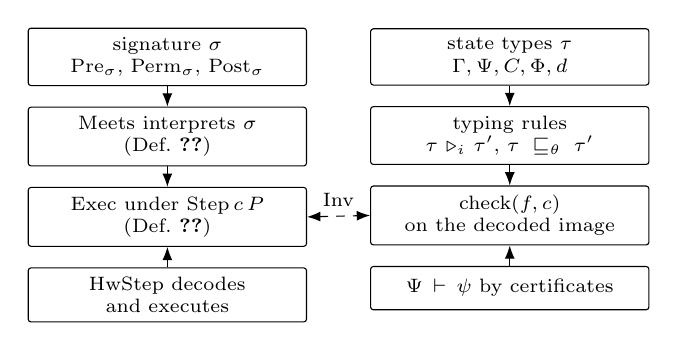
\begin{tikzpicture}[font=\scriptsize,>=Latex,node distance=2.6mm,
 box/.style={draw,rounded corners=1pt,align=center,minimum height=5.5mm,text width=33mm}]
\node[box] (sig) {signature $\sigma$\\ $\Pre_\sigma$, $\Perm_\sigma$, $\Post_\sigma$};
\node[box,below=of sig] (meets) {$\Meets$ interprets $\sigma$\\ (Def.~\ref{def:meets})};
\node[box,below=of meets] (exec) {$\Exec$ under $\Step\,c\,P$\\ (Def.~\ref{def:exec})};
\node[box,below=of exec] (hw) {$\HwStep$ decodes and executes};
\node[box,right=8mm of sig] (ty) {state types $\tau$\\ $\Gamma,\Psi,C,\Phi,d$};
\node[box,below=of ty] (rules) {typing rules\\ $\tau\triangleright_i\tau'$, $\tau\sub{\theta}\tau'$};
\node[box,below=of rules] (chk) {$\chk(f,c)$\\ on the decoded image};
\node[box,below=of chk] (q) {$\Psi\ent\psi$ by certificates};
\draw[->] (sig)--(meets); \draw[->] (meets)--(exec); \draw[->] (hw)--(exec);
\draw[->] (ty)--(rules); \draw[->] (rules)--(chk); \draw[->] (q)--(chk);
\draw[<->,dashed] (exec.east)--node[above]{$\Inv$}(chk.west);
\end{tikzpicture}
\caption{Concrete semantics (left) and static semantics (right), joined by the invariant $\Inv$ (Definition~\ref{def:inv}). Theorem~\ref{thm:check} turns $\chk(f,c)=\mathit{true}$ into $\Meets$.}
\Description{Two columns: signatures, Meets, Exec, and the hardware step on the left; state types, typing rules, the checker, and entailment on the right; a dashed arrow labelled Inv joins Exec and the checker.}
\label{fig:overview}
\end{figure}

\paragraph{Contributions.}
\begin{itemize}
\item A type language for machine code with linear index expressions modulo $2^{64}$, byte capabilities with fields, opaque tokens, and ownership transfer, in which safe and unsafe functions share one signature form (Sections~\ref{sec:static} and~\ref{sec:sigs}).
\item The meaning $\sem{\sigma}$ as a total-correctness judgment over a RISC-V semantics with byte-granular permissions, and its partial variant (Section~\ref{sec:sigs}).
\item Typing rules for the full integer instruction set of the profile, stack frames, calls, compiler call sequences, and system calls, and a checker that re-checks an untrusted per-instruction record on the decoded image (Sections~\ref{sec:rules} and~\ref{sec:checker}).
\item Machine-checked soundness of that checker, a program-level composition theorem, and transfer to the hardware step, all in Lean with standard axioms only (Sections~\ref{sec:soundness}--\ref{sec:hw}).
\item An evaluation on unmodified compiler output of musl libc, with verdicts predicted before compiling (Section~\ref{sec:eval}).
\end{itemize}
Each definition and theorem names its Lean counterpart; the development is available at the commit cited as~\cite{nocompiler}.

\paragraph{Running example.} Fig.~\ref{fig:sum} shows the function \code{sum}, which adds $n$ 64-bit words from address $\rho$, as \code{clang -O2} emits it, with a signature and one loop annotation in assembler comments. We use it throughout the paper. We present its signature in Example~\ref{ex:sig}, its meaning in Example~\ref{ex:meets}, its loop-head type in Example~\ref{ex:tau}, its load in Example~\ref{ex:load}, its back edge and ranking function in Example~\ref{ex:back}, and its theorem in Example~\ref{ex:final}.

\begin{figure*}[t]
\begin{alltt}\small
#: fn sum [\(\rho\), n]  in a0: int(\(\rho\)), a1: int(n)
#:   borrow \(\rho\) \(\mapsto\) bytes[8n] ro   where 8 \(\mid\) \(\rho\)   out a0: int
0  sum:    li   a2, 0
1          beqz a1, .LBB0_2
2  .LBB0_1:  #: inv [m] a0: int(\(\rho\)+8n\(-\)8m), a1: int(m) where 1\(\le\)m\(\le\)n decreases m
2          ld   a3, 0(a0)
3          add  a2, a3, a2
4          addi a1, a1, -1
5          addi a0, a0, 8
6          bnez a1, .LBB0_1
7  .LBB0_2:  mv   a0, a2
8          ret
\end{alltt}
\vspace{-4pt}
\caption{The running example shows compiler output with annotations in \texttt{\#:} comments. The left column is the instruction index $k$; the instruction at $k$ lies at address $e+4k$.}
\Description{An RV64 assembly listing of sum with its signature and loop invariant.}
\label{fig:sum}
\end{figure*}

%======================================================================
\section{Concrete semantics}\label{sec:concrete}
We give mathematical types rather than the exact Lean data-structure encodings. Auxiliary names introduced here are presentation-level notation unless explicitly identified with a Lean definition. In particular, lists, finite maps, and address sets are used to expose the logical content of the definitions. Partial functions are written with $\rightharpoonup$, and optional results with $\Opt$. Where a Boolean checker appears as a proposition, it denotes equality to $\mathit{true}$. We retain the Lean names to identify the corresponding formal definitions.
Throughout, $B=2^{64}$, $\W=\{0,1\}^{64}$, and $\un{w}\in[0,B)$ is the unsigned value of a word $w$. Addresses are words, and address arithmetic is modulo $B$.

\begin{definition}[Machine state and code image; \lean{State}, \lean{Code}]\label{def:state}
Let $\Ty{Reg}=\{0,\ldots,31\}$, $\Ty{Byte}=\{0,1\}^8$, $\Ty{Word32}=\{0,1\}^{32}$ and $\Ty{Memory}=\W\to\Ty{Byte}$. We use $\Ty{Event}$ for the abstract type of observable system-call events and $\Ty{ExitCode}$ for the abstract type of process exit codes. These two payload types are left abstract in this presentation; the environment model supplies their concrete representation. The state and code-image types are
\[
\begin{aligned}
\Ty{State}&=\{s\in\Ty{RawState}\mid s.R(0)=0\},\\
\Ty{RawState}&=\W\times(\Ty{Reg}\to\W)\times\Ty{Memory}\\ &\quad\times\List(\Ty{Event})\times\Opt(\Ty{ExitCode}),\\
pc&\in\W,\quad R\in\Ty{Reg}\to\W,\quad M\in\Ty{Memory},\\
E&\in\List(\Ty{Event}),\quad X\in\Opt(\Ty{ExitCode}),\\
\Ty{Code}&=\W\times\List(\Ty{Word32}).
\end{aligned}
\]
We write $s.pc,s.R,s.M,s.E,s.X$ for the projections of a state and $c.base,c.words$ for those of a code image. The event trace records observable interactions with the execution environment. An exit status of $\mathrm{none}$ means that the process is running. Let $\Ty{Instr}$ denote the decoded instructions supported by the model. Define
\[
\begin{aligned}
\mathrm{decode}&:\Ty{Word32}\to\Opt(\Ty{Instr}),\\
c.\mathit{instr}&:\W\to\Opt(\Ty{Instr}),\\
c.\mathit{instr}(a)&=
\begin{cases}
\mathrm{decode}(c.words[k]) & 4\mid d\ \land\ k<|c.words|,\\
\mathrm{none}&\text{otherwise},
\end{cases}\\
 d&=\un{a-c.base},\qquad k=\lfloor d/4\rfloor.
\end{aligned}
\]
The code image is immutable during the abstract execution, whereas the memory in a state can change. For an optional result, we abbreviate equality to its successful constructor by writing an equality such as $c.\mathit{instr}(a)=i$.
\end{definition}

\paragraph{Example.} If $c.base=\mathtt{0x1000}$ and $c.words=[\mathtt{0x00500093},\mathtt{0x00008067}]$, then $c.\mathit{instr}(\mathtt{0x1000})$ decodes to \code{addi x1,x0,5}, and $c.\mathit{instr}(\mathtt{0x1004})$ decodes to \code{jalr x0,0(ra)}. The address \texttt{0x1001} is not an instruction boundary, so its result is \textsf{none}.


The decoder (\lean{Isa.lean}) supports the modeled RV64I, M, Zba, and Zbb encodings~\cite{riscvspec}, although compressed, atomic, floating-point, CSR, and fence instructions decode to nothing. RV64I provides the basic 64-bit integer instructions. M adds multiplication and division, Zba adds address-generation operations, and Zbb adds basic bit manipulation. An encoder and the theorem \lean{decode\_encode} relate the two directions. $\mathit{exec}(i,s)$ (\lean{Machine.lean}) is the effect of instruction $i$; it is undefined on a misaligned access and on a jump to an address that is not a multiple of four. System calls are a relation $\mathrm{Sys}(s,s')$ (\lean{Env.lean}) for \code{read}, \code{write}, \code{exit}, and \code{exit\_group}: a \code{write} of $n\ge1$ bytes either fails with $-e$, $1\le e\le4095$, or transfers $1\le r\le\min(n,\mathtt{0x7ffff000})$ bytes and appends an event; system calls outside the four modeled calls have no successor.

\begin{definition}[Hardware step; \lean{HwStep}]\label{def:hwstep}
The ordinary instruction semantics is a partial function $\mathit{exec}:\Ty{Instr}\times\Ty{State}\rightharpoonup\Ty{State}$. The environment semantics is a relation $\mathrm{Sys}:\Ty{State}^2\to\Prop$. For $w\in\{4,8\}$, let $\mathrm{load}_{8w}:\Ty{Memory}\times\W\to\{0,1\}^{8w}$ read a little-endian word. Its unsigned value is $\sum_{j=0}^{w-1}2^{8j}\un{M(a+j)}$, where the byte addresses are computed modulo $B$. For $i\in\Ty{Instr}$ define
\[
\begin{aligned}
\mathrm{RunInstr}(i,s,s')\iff{}& (i\ne\mathtt{ecall}\land\mathit{exec}(i,s)=s')\\
 &\lor(i=\mathtt{ecall}\land\mathrm{Sys}(s,s')).
\end{aligned}
\]
The hardware step $\HwStep:\Ty{State}^2\to\Prop$ is the relation
\[
\begin{aligned}
\HwStep(s,s')\iff{}& s.X=\mathrm{none}\land 4\mid\un{s.pc}\\
&\land\exists i\in\Ty{Instr}.\ \mathrm{decode}(\mathrm{load}_{32}(s.M,s.pc))=i\\
&\hspace{26mm}\land\mathrm{RunInstr}(i,s,s').
\end{aligned}
\]
\end{definition}
Ordinary instructions have at most one result in this model. System calls can have multiple results because the environment can choose the bytes returned by a read or the amount transferred. For example, an aligned \code{add x3,x1,x2} updates register $3$ to $s.R(1)+s.R(2)$ modulo $B$ and advances the PC by four. A read can instead produce distinct successor memories even when its initial state is fixed.

\subsection{Permissions}
We represent a region by $r\in\Ty{Region}=\W\times\N$. Its address set is $A(r)=\{x\in\W\mid\un{x-r.base}<r.size\}$. We extend $A$ to lists of regions by taking the union of their address sets. Because subtraction is modulo $B$, a region may wrap around the address space.

\begin{definition}[Permission; \lean{Perm}, \lean{Perm.canRead}]\label{def:perm}
The type of permissions is $\Ty{Perm}=\List(\Ty{Region})\times\List(\Ty{Region})$. For $P=(P.rd,P.wr)$ and $x\in\W$, define
\[
\begin{aligned}
\mathrm{readable}(P,x)&\iff x\in A(P.rd)\cup A(P.wr),\\
\mathrm{writable}(P,x)&\iff x\in A(P.wr),\\
\canRead(P,a,n)&\iff\forall j\in\N.\ j<n\Rightarrow\mathrm{readable}(P,a+j),\\
\canWrite(P,a,n)&\iff\forall j\in\N.\ j<n\Rightarrow\mathrm{writable}(P,a+j).
\end{aligned}
\]
The first two predicates have type $\Ty{Perm}\times\W\to\Prop$, and the last two have type $\Ty{Perm}\times\W\times\N\to\Prop$. Permission inclusion is
\[
\begin{aligned}P\le Q\iff{}& A(P.rd)\cup A(P.wr)\\ &\subseteq A(Q.rd)\cup A(Q.wr)\\ &\land A(P.wr)\subseteq A(Q.wr).\end{aligned}
\]
\end{definition}

\paragraph{Example.} With $P.rd=[(100,8)]$ and $P.wr=[(108,8)]$, $\canRead(P,104,8)$ holds because all eight bytes are readable. In contrast, $\canWrite(P,104,8)$ does not hold because the first four bytes lack write permission.


The judgment is byte-wise, so an access need not lie in one region. This matters for ownership transfer, where a capability returned by a callee may span two regions of the receiver's permission (Section~\ref{sec:calls}).

\begin{definition}[Permitted step; \lean{Step}]\label{def:step}
Define $\mathrm{AccessOk}:\Ty{Perm}\times\Ty{Instr}\times\Ty{State}\to\Prop$. For ordinary instructions, let $a$ be the effective address computed in $s$ and $w$ the byte width, whenever the instruction accesses memory. For system calls let $b=s.R(a_1)$ and $n=\un{s.R(a_2)}$.
\[
\begin{gathered}\mathrm{AccessOk}(P,i,s)\iff\\[-2pt]\begin{cases}
\canRead(P,a,w)&i\text{ is a load},\\
\canWrite(P,a,w)&i\text{ is a store},\\
\canRead(P,b,n)&\text{write system call},\\
\canWrite(P,b,n)&\text{read system call},\\
\top&\text{otherwise}.\end{cases}\end{gathered}
\]
The relation $\Step:\Ty{Code}\times\Ty{Perm}\times\Ty{State}^2\to\Prop$ is
\[
\begin{aligned}
\Step(c,P,s,s')\iff{}&s.X=\mathrm{none}\land\exists i\in\Ty{Instr}.\\
 &c.\mathit{instr}(s.pc)=i\\ &\land\mathrm{RunInstr}(i,s,s')\\ &\land\mathrm{AccessOk}(P,i,s).
\end{aligned}
\]
\end{definition}

\paragraph{Example.} For \code{ld a3,0(a0)} with $s.R(a_0)=104$, the checker requires $\canRead(P,104,8)$ in addition to the instruction's execution semantics. The permission in the preceding example meets this condition. In contrast to $\HwStep$, the instruction is fetched from $c$ rather than from $s.M$.


The instruction comes from the image, not from memory; the two agree when the image is loaded, its base is aligned, and no writable byte overlaps it (Section~\ref{sec:hw}). A nonfinal state with no $\Step$ successor is stuck. This can result from a fault, an access outside $P$, an undecodable word, or an unmodeled system call.

\subsection{Executions}
A domain $D\in\Ty{Domain}=\List(\Ty{Region})$ specifies the code ranges under consideration. We abbreviate $s.pc\in A(D)$ by $s.pc\in D$ and define $\Final_D:\Ty{State}\to\Prop$ by
\[\Final_D(s)\iff s.pc\notin D\lor s.X\ne\mathrm{none}.\]

\begin{definition}[Reach and Exec; \lean{Reach}, \lean{Exec}]\label{def:exec}
Both $\Reach$ and $\Exec$ have type
\[\Ty{Code}\times\Ty{Perm}\times\Ty{Domain}\times(\Ty{State}\to\Prop)\to(\Ty{State}\to\Prop).\]
For fixed $c,P,D,Q$, $\Reach(c,P,D,Q)$ is the least inductively generated predicate on states closed under the following two rules.
\begin{mathpar}
\inferrule{Q(s)}{\Reach(c,P,D,Q)(s)}
\and
\inferrule{s.pc\in D \\ \exists s'.\,\Step(c,P,s,s') \\ \forall s'.\ \Step(c,P,s,s')\Rightarrow\Reach(c,P,D,Q)(s')}{\Reach(c,P,D,Q)(s)}
\end{mathpar}
We then define the total execution predicate by
\[\Exec(c,P,D,Q)(s)\triangleq\Reach(c,P,D,\lambda t.\,\Final_D(t)\land Q(t))(s).\]
\end{definition}

\paragraph{Example.} Suppose a state has two permitted successors. If both successors satisfy the goal, and the initial PC is in $D$, then the second rule establishes $\Reach$ of the initial state. If one successor is stuck before satisfying the goal, the rule cannot establish it. For $\Exec$, the goal additionally requires that the PC has left $D$ or that the process has exited.


Because $\Reach$ is inductive, $\Exec(c,P,D,Q)(s)$ requires that every permitted execution from $s$ progresses until it reaches a final state after finitely many steps and that $Q$ holds at that state. In particular, a nonfinal state cannot be stuck. This property concerns the permitted-step model; Theorem~\ref{thm:hw} subsequently transfers it to hardware steps under additional assumptions. Every choice of the environment (how many bytes a \code{write} accepts, what a \code{read} returns) is covered. The formal development proves monotonicity, sequential composition into a larger domain and permission (\lean{Reach.bind}), invariants, a loop rule with a decreasing measure, and a frame property, by which memory outside the writable bytes of $P$ is unchanged (\lean{VerifiedImg.frame}).

\begin{definition}[Partial execution; \lean{ReachP}, \lean{ExecP}]\label{def:execp}
The type of $\mathrm{ReachP}$ is $\Ty{Code}\times\Ty{Perm}\times\Ty{Domain}\times(\Ty{State}\to\Prop)\times\N\to(\Ty{State}\to\Prop)$. Fix $c,P,D,Q$ and abbreviate its value at index $n$ by $R_n(s)$. Its recursive equations are
\[
\begin{aligned}
R_0(s)&\iff\top,\\
R_{n+1}(s)&\iff Q(s)\lor\big(s.pc\in D\land (\exists t.\ \Step(c,P,s,t))\\
&\hspace{27mm}\land (\forall t.\ \Step(c,P,s,t)\Rightarrow R_n(t))\big).
\end{aligned}
\]
The partial execution predicate has the same type as $\Exec$ and is defined by
\[\begin{aligned}\Exec^{\mathrm p}(c,P,D,Q)(s)\iff{}&\forall n\in\N.\\ &\mathrm{ReachP}(c,P,D,\\ &\quad\lambda t.\ \Final_D(t)\land Q(t),n)(s).\end{aligned}\]
\end{definition}

This predicate asserts safety of every finite prefix and the postcondition whenever execution reaches a final state. It does not require termination. For example, a valid jump to itself inside $D$ satisfies $\Exec^{\mathrm p}$ by induction on the index, but does not satisfy $\Exec$ if no final state is reached.
\begin{figure*}[t]
\centering
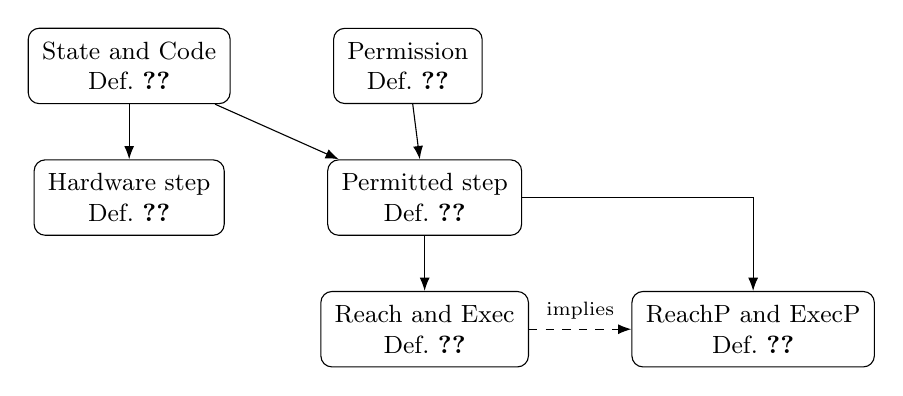
\begin{tikzpicture}[>=Latex, node distance=7mm and 13mm, every node/.style={font=\small}, b/.style={draw,rounded corners,align=center,inner sep=5pt}]
\node[b] (s) {State and Code\\Def.~\ref{def:state}};
\node[b,right=of s] (p) {Permission\\Def.~\ref{def:perm}};
\node[b,below=of s] (h) {Hardware step\\Def.~\ref{def:hwstep}};
\node[b,right=of h] (st) {Permitted step\\Def.~\ref{def:step}};
\node[b,below=of st] (e) {Reach and Exec\\Def.~\ref{def:exec}};
\node[b,right=of e] (ep) {ReachP and ExecP\\Def.~\ref{def:execp}};
\draw[->] (s)--(h); \draw[->] (s)--(st); \draw[->] (p)--(st); \draw[->] (st)--(e); \draw[->] (st.east)-| (ep.north); \draw[->,dashed] (e)--node[above,font=\scriptsize]{implies} (ep);
\end{tikzpicture}
\caption{The concrete definitions share the instruction semantics. The permitted step additionally uses the fixed image and permission. Total execution implies partial execution. The hardware connection requires the hypotheses of Theorem~\ref{thm:hw}.}
\Description{A dependency graph for the concrete semantics.}
\end{figure*}


%======================================================================
\section{Static semantics}\label{sec:static}
\begin{definition}[Index expressions and constraints; \lean{IExpr}, \lean{Constr}, \lean{Val}]\label{def:index}
Let $\Ty{Var}=\N$ and $\Ty{Val}=\Ty{Var}\to\Z$. An index expression belongs to the set of finite linear integer expressions
\[\Ty{IExpr}=\{c_0+\textstyle\sum_{j=1}^m c_jx_j\mid m\in\N,\ c_j\in\Z,\ x_j\in\Ty{Var}\}.\]
Evaluation has type $\Ty{IExpr}\times\Ty{Val}\to\Z$ and satisfies $\ev{e}{\iota}=c_0+\sum_j c_j\iota(x_j)$. The constraint type $\Ty{Constr}$ has grammar
\[\psi::=\top\mid\bot\mid e_1\le e_2\mid e_1=e_2\mid c\mid e\mid\psi\land\psi\mid\psi\lor\psi\mid\lnot\psi,\quad c\in\Z_{>0}.\]
The satisfaction relation $\models\ \subseteq\Ty{Val}\times\Ty{Constr}$ is defined recursively by
\[
\begin{aligned}
\iota\models\top&\iff\top,\\ \iota\models\bot&\iff\bot,\\
\iota\models(e_1\le e_2)&\iff\ev{e_1}{\iota}\le\ev{e_2}{\iota},\\ 
\iota\models(e_1=e_2)&\iff\ev{e_1}{\iota}=\ev{e_2}{\iota},\\
\iota\models(c\mid e)&\iff\ev{e}{\iota}\bmod c=0,\\
\iota\models(\psi_1\land\psi_2)&\iff(\iota\models\psi_1)\land(\iota\models\psi_2),\\
\iota\models(\psi_1\lor\psi_2)&\iff(\iota\models\psi_1)\lor(\iota\models\psi_2),\\
\iota\models\lnot\psi&\iff\lnot(\iota\models\psi).
\end{aligned}
\]
For $\Psi\in\List(\Ty{Constr})$, define $\iota\models\Psi\iff\forall\psi\in\Psi.\ \iota\models\psi$. We abbreviate $B\mid(e_1-e_2)$ by $e_1\eqB e_2$.
\end{definition}

\paragraph{Example.} If $\iota(x)=100$, $\iota(y)=8$ and $\iota(z)=3$, then $\ev{x+8y-8z}{\iota}=140$. The constraint $z\le y$ holds under this valuation. A product $xy$ is not an index expression unless one factor is a constant.


Index variables are logical rather than machine registers. The proof preserves input variables and uses fresh variables or substitutions to interpret successive state types. Constraints are quantifier-free Presburger formulas, so their validity is decidable.

\begin{definition}[Value type; \lean{HasInt}]\label{def:hasint}
The value-type judgment $\mathrm{HasInt}:\W\times\Ty{Val}\times\Ty{IExpr}\to\Prop$ is written $w\models_\iota\inttype{e}$ and is defined by
\[
\boxed{\;w\models_\iota\inttype{e}\iff\un{w}\equiv\ev{e}{\iota}\pmod{B}.\;}
\]
\end{definition}

\paragraph{Example.} If $w=B-1$ has type $\inttype{x}$ under $\iota(x)=B-1$, then adding one produces the machine word $0$, which has type $\inttype{x+1}$ because $0\equiv B\pmod B$. The congruence is therefore essential for tracking wrapping arithmetic without imposing a no-overflow condition.


Because the type is a congruence, the results of \code{add}, \code{sub}, shifts, and multiplication by constants have exact types without overflow conditions. Order matters at comparisons and accesses, so the checker introduces the \emph{unsigned representative} $u(e)$, which is $e$ itself when $0\le e<B$ is entailed, and otherwise a fresh variable $x$ with $0\le x<B$ and $x\eqB e$; the signed representative $s(e)$ is analogous on $[-2^{63},2^{63})$ (\lean{STy.urep}, \lean{STy.srep}). A pointer is an index expression like any other, e.g.\ $\inttype{\rho+8k}$; it carries no permission.

\subsection{Capabilities}
\begin{definition}[Capabilities; \lean{Cap}, \lean{BytesCap}, \lean{Field}]\label{def:cap}
Let $\Ty{TokenName}$ be the abstract type of token names and let $\Ty{Mode}=\{\mathsf{ro},\mathsf{rw}\}$. A field is a pair $(k,e)\in\Ty{Field}=\N\times\Ty{IExpr}$ and describes an eight-byte word at offset $k$. The capability types are
\[
\begin{aligned}
\Ty{BytesCap}&=\Ty{IExpr}^2\times\Ty{Mode}\times\Ty{Bool}\times\List(\Ty{Field}),\\
\Ty{CapKind}&=\Ty{BytesCap}\uplus\Ty{TokenName},\\
\Ty{Cap}&=\Ty{Constr}\times\Ty{CapKind}.
\end{aligned}
\]
We write a capability as $\psi\Rightarrow\kappa$, where $\psi$ is its guard and the kind $\kappa$ has one of the following forms.
\[\kappa::=\bytes{b}{n}{m}\,[\mathsf{heap}]\,\{k_1{:}\inttype{e_1},\ldots\}\mid\mathsf{tok}(t).\]
The Boolean marker indicates whether the byte range must be a live heap allocation unit. The exclusivity predicate is true exactly for a byte capability with mode $\mathsf{rw}$ or a token capability. A false guard makes the capability inactive.
\end{definition}

\paragraph{Example.} The capability $\top\Rightarrow\bytes{b}{24}{rw}\{0{:}\inttype{x},8{:}\inttype{y}\}$ grants access to 24 bytes starting at $b$ and records the values of the first two eight-byte fields. It makes no assertion about the contents of the last eight bytes.


\begin{definition}[Footprint, validity; \lean{Cap.fp}, \lean{Cap.valid}]\label{def:valid}
Let $\Ty{TokenMeanings}=\Ty{TokenName}\to\Ty{TokDef}$ and $\Ty{TokenFootprints}=\Ty{TokenName}\to\List(\Ty{Region})$. Token definitions are specified in Definition~\ref{def:tok}. Fix $T\in\Ty{TokenMeanings}$, $F\in\Ty{TokenFootprints}$ and $\iota\in\Ty{Val}$. We view footprints as address sets, with type $\fp_{\iota,F}:\Ty{Cap}\to\mathcal P(\W)$. In the following formulas we use integer intervals as shorthand for their word addresses when the byte capability is valid. The exact representation of footprints for invalid capabilities is not needed for these explanations and is determined by the Lean definition. For valid byte capabilities this interval never wraps. Define
\[
\begin{gathered}\fp_{\iota,F}(\psi\Rightarrow\kappa)=\\[-2pt]\begin{cases}
\emptyset&\iota\not\models\psi,\\
[\ev{b}{\iota},\ev{b}{\iota}+\ev{n}{\iota})&\substack{\iota\models\psi,\\ \kappa=\bytes{b}{n}{m}\ldots},\\
A(F(t))&\iota\models\psi,\ \kappa=\mathsf{tok}(t).\end{cases}\end{gathered}
\]
The relation $\Valid_{T,\iota,F}:\Ty{Memory}\times\Ty{Cap}\to\Prop$ is defined using an auxiliary predicate $V$ on capability kinds.
\[
\Valid_{T,\iota,F}(M,\psi\Rightarrow\kappa)\iff(\iota\not\models\psi)\lor V(M,\kappa).
\]
For a byte capability $k_b$ with fields $(k_j,e_j)$, let $b_0=\ev{b}{\iota}$ and $n_0=\ev{n}{\iota}$. Then
\[
\begin{aligned}
V(M,k_b)\iff{}&0\le b_0\land0\le n_0\land b_0+n_0\le B\\
&\land\bigwedge_j\big(k_j+8\le n_0\land8\mid(b_0+k_j)\\
&\quad\land\mathrm{load}_{64}(M,b_0+k_j)\models_\iota\inttype{e_j}\big)\\
&\land( k_b.\mathit{heap}\Rightarrow\\ &\qquad T(\mathsf{Heap}).\mathit{unit}(F(\mathsf{Heap}),(b_0,n_0))).\\
V(M,\mathsf{tok}(t))\iff{}&T(t).\mathit{inv}(F(t),M).
\end{aligned}
\]
Here $\mathrm{load}_{64}$ reads eight consecutive bytes as a word. The range conditions ensure that the indicated byte addresses are representable, and the field conditions connect the memory contents to Definition~\ref{def:hasint}.
\end{definition}

\paragraph{Example.} For $\iota(b)=104$ and $n=16$, the footprint is $\{104,\ldots,119\}$. A field at offset 8 is valid if the word at address 112 has the declared type. A field at offset 12 cannot be valid because $12+8>16$, irrespective of the memory contents.


A field is a fact about memory contents rather than a permission. Therefore, using an address stored in a field requires a separate capability for the bytes to which it points. A structure holding a pointer and a length is therefore a capability with two fields next to a second capability for the buffer.

\begin{definition}[Token meaning; \lean{TokDef}]\label{def:tok}
A token meaning $t_d\in\Ty{TokDef}$ comprises the following two relations and a proof of locality.
\[
\begin{aligned}
t_d.\mathit{inv}&:\List(\Ty{Region})\times\Ty{Memory}\to\Prop,\\
t_d.\mathit{unit}&:\List(\Ty{Region})\times\Ty{Region}\to\Prop.
\end{aligned}
\]
The locality proof establishes
\[
\begin{aligned}&\forall R,M,M'.\quad\big(\forall a\in A(R).\ M(a)=M'(a)\big)\\ &\quad\land t_d.\mathit{inv}(R,M)\Rightarrow t_d.\mathit{inv}(R,M').\end{aligned}
\]
The unit relation describes the live allocation units for the given footprint and is empty by default. The allocator's token is named $\mathsf{Heap}$.
\end{definition}

\paragraph{Example.} An allocator may choose an invariant describing its private metadata. If a store changes only bytes outside its footprint, locality preserves that invariant without exposing the allocator's representation. The exact allocator invariant and unit relation are supplied by its token meaning, not fixed by this definition.


\begin{definition}[Separation; \lean{Separated}]\label{def:sep}
The separation predicate has type $\Ty{Val}\times\Ty{TokenFootprints}\times\List(\Ty{Cap})\to\Prop$. For $C=[\kappa_1,\ldots,\kappa_m]$, define
\[
\begin{aligned}\Sep_{\iota,F}(C)\iff{}&\forall i,j\in\{1,\ldots,m\}.\\ &(i\ne j\land\mathrm{exclusive}(\kappa_i))\\ &\Rightarrow\fp_{\iota,F}(\kappa_i)\cap\fp_{\iota,F}(\kappa_j)=\emptyset.\end{aligned}
\]
Because the ordered pairs include both orientations, an overlap is forbidden whenever either capability is exclusive. Read-only footprints may overlap each other.
\end{definition}

\paragraph{Example.} The ranges $[100,116)$ and $[108,124)$ may coexist if both are read-only. If either is writable, their intersection $[108,116)$ violates separation. Consequently a store through one writable capability cannot invalidate a field or token invariant belonging to another held capability.


Separation removes the need to analyze aliases between exclusive and other held capabilities because a store through an exclusive capability cannot modify the bytes or fields of any other held capability.

\subsection{State types}
\begin{definition}[State type; \lean{STy}, \lean{HCap}]\label{def:sty}
Let $\Ty{Id}$ denote capability identities and $\Ty{Offset}$ denote stack-slot offsets. A held capability includes its capability, identity and optional origin in the signature.
\[
\Ty{HCap}=\Ty{Cap}\times\Ty{Id}\times\Opt(\N).
\]
A state type $\tau=(\Gamma,\Psi,C,\Phi,d)$ belongs to $\Ty{STy}$, whose components have the following types.
\[
\begin{aligned}
\Gamma&:\Ty{Reg}\rightharpoonup\Ty{IExpr},&\Psi&\in\List(\Ty{Constr}),\\
C&\in\List(\Ty{HCap}),&\Phi&:\Ty{Offset}\rightharpoonup\Ty{IExpr},\\
d&\in\N.
\end{aligned}
\]
An absent register or slot is unconstrained. Let $U(C)$ be the list of pairs $(b,n)$ extracted from held byte capabilities with guard $\top$. The hypothesis list is
\[\mathrm{hyps}(\tau)=\tau.\Psi\mathbin{+\!+}\mathop{\mathrm{concat}}_{(b,n)\in U(\tau.C)}[0\le b,\ 0\le n,\ b+n\le B].\]
Here $+\!+$ denotes list concatenation. The additional facts follow from capability validity rather than from a new assumption about the machine.
\end{definition}

\paragraph{Example.} At the head of the running loop, $\Gamma(a_0)=\rho+8n-8m$ and $\Gamma(a_1)=m$. The facts include $1\le m\le n$, while $C$ contains the readable array of $8n$ bytes. If the function also saved $ra$ at stack offset 24 in a 32-byte frame, $\Phi(24)$ would record its symbolic value and $d$ would be 32. The running example itself uses no stack frame.
\begin{figure*}[t]
\centering
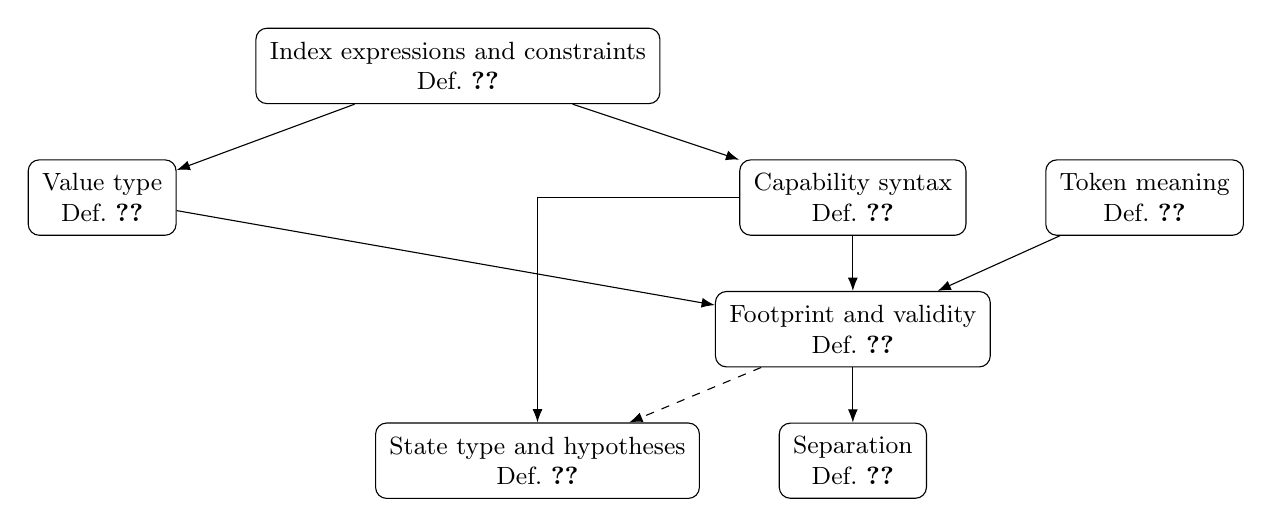
\begin{tikzpicture}[>=Latex,node distance=7mm and 10mm,b/.style={draw,rounded corners,align=center,font=\small,inner sep=5pt}]
\node[b] (ix) {Index expressions and constraints\\Def.~\ref{def:index}};
\node[b,below left=of ix] (int) {Value type\\Def.~\ref{def:hasint}};
\node[b,below right=of ix] (cap) {Capability syntax\\Def.~\ref{def:cap}};
\node[b,right=of cap] (tok) {Token meaning\\Def.~\ref{def:tok}};
\node[b,below=of cap] (val) {Footprint and validity\\Def.~\ref{def:valid}};
\node[b,below=of val] (sep) {Separation\\Def.~\ref{def:sep}};
\node[b,left=of sep] (sty) {State type and hypotheses\\Def.~\ref{def:sty}};
\draw[->] (ix)--(int); \draw[->] (ix)--(cap); \draw[->] (cap)--(val); \draw[->] (int)--(val); \draw[->] (tok)--(val); \draw[->] (val)--(sep); \draw[->] (cap.west)-| (sty.north); \draw[->,dashed] (val)--(sty); 
\end{tikzpicture}
\caption{The static language uses index expressions in value types and capabilities. Validity interprets capabilities against memory, while separation constrains their joint footprints. State types record the information that the checker manipulates.}
\Description{A dependency graph of the static semantics.}
\end{figure*}


The added hypotheses follow from validity, which ensures that an active byte capability lies in the address space. An access proved to be inside that range consequently does not wrap.

%======================================================================
\section{Entailment}\label{sec:entail}
The checker must establish entailments $\Psi\ent\psi$, which require every valuation satisfying $\Psi$ to satisfy $\psi$. The checker attempts to establish them by refuting $\Psi\land\lnot\psi$.

\begin{definition}[Certificates; \lean{Cert}, \lean{Query.check}]\label{def:cert}
Let $\Ty{Lin}=\Ty{IExpr}$, where a form $l=c+\sum_j a_jx_j$ represents the inequality $l\ge0$. A certificate is a finite list of instructions of three kinds. The operands of a combination or tightening instruction refer to earlier steps.
\[
\begin{aligned}
\Ty{CertStep}::={}&\mathsf{hyp}(j)\mid\mathsf{add}(j,k,p,q)\mid\mathsf{tighten}(j),\\
&j,k,p,q\in\N,\qquad \Ty{Cert}=\List(\Ty{CertStep}).
\end{aligned}
\]
For hypotheses $H\in\List(\Ty{Lin})$, the step evaluator checks indices and computes forms using the following rules.
\begin{mathpar}
\inferrule{l\in H}{l\ge0}\and
\inferrule{l_1\ge0\\ l_2\ge0\\p,q\in\N}{pl_1+ql_2\ge0}\and
\inferrule{c+\sum_j a_jx_j\ge0\\g=\gcd_j(a_j)>0}{\lfloor c/g\rfloor+\sum_j(a_j/g)x_j\ge0}
\end{mathpar}
Let $\mathrm{evalCert}(H,cs)$ denote the optional list of resulting forms. The refutation predicate holds when evaluation succeeds and at least one resulting form is a negative constant.
\[\mathrm{Refutes}(H,cs)\iff\exists L.\ \mathrm{evalCert}(H,cs)=L\land\exists k\in\Z_{>0}.\ -k\in L.\]
A query has type $\Ty{Query}=\List(\Ty{Constr})\times\Ty{Constr}$, and its semantics is
\[\Psi\ent\psi\iff\forall\iota\in\Ty{Val}.\ \iota\models\Psi\Rightarrow\iota\models\psi.\]
To verify this judgment, the checker converts $\Psi\land\lnot\psi$ into disjunctive normal form and linearizes each disjunct. Divisibility $c\mid e$ becomes $e=cq$, while its negation becomes $e=cq+r$ with $1\le r\le c-1$, using fresh variables. Equalities are represented by two inequalities. These transformations preserve satisfiability under extension of valuations. Write $[H_1,\ldots,H_m]$ for the resulting list of lists of linear forms. The Boolean checker satisfies
\[\begin{aligned}&\mathrm{check}((\Psi,\psi),cs)=\mathit{true}\\ &\iff |cs|=m\land\forall j\in\{1,\ldots,m\}.\\ &\qquad\mathrm{Refutes}(H_j,cs_j).\end{aligned}\]
The certificate syntax here describes the mathematical operations rather than the exact serialization of Lean constructors.
\end{definition}

\paragraph{Example.} To show $x\ge3\ent x\ge2$, the negated goal gives $x\le1$. The forms $x-3$ and $1-x$ add to the negative constant $-2$. Tightening can also derive $x-2\ge0$ from $2x-3\ge0$ because $x$ is integral. The checker validates each step without trusting the search algorithm.


\begin{claim}[Soundness of entailment; \lean{Query.check\_sound}, \lean{Query.decide\_sound}]\label{thm:entail}
If $\mathrm{check}(q,\mathit{cs})$, then every valuation satisfying the hypotheses of $q$ satisfies its goal. Consequently $\mathrm{decide}(q)$, which runs an untrusted Fourier--Motzkin search for certificates and checks them, satisfies $\mathrm{decide}(q)=\mathit{true}\Rightarrow\Psi\models\psi$.
\end{claim}
\begin{proof}[Proof sketch]
Each step derives a form that is non-negative under every valuation of the extended variables satisfying the disjunct; tightening is sound because the left side is an integer. A negative constant is then a contradiction. The fresh-variable translation preserves satisfiability under an extension of the valuation (\lean{linsOf\_sound}), and the DNF covers every model of the formula (\lean{Constr.dnf\_complete}).
\end{proof}

The search is incomplete because it stops when it reaches its fuel or size limits. Incompleteness can only cause a rejection. The checker's entailment $\tau\ent\psi$ (\lean{STy.ent}) passes to $\mathrm{decide}$ the hypotheses of $\tau$ that share variables with $\psi$, directly or through other hypotheses; dropping hypotheses is sound.

\begin{example}[The \code{beqz} edge of \code{sum}]\label{ex:beq}
On the fall-through edge of \code{beqz a1} the checker adds $\lnot(n\eqB0)$. With $0\le 8n$ and $\rho+8n\le B$ from the capability and $\rho\ge0$, it proves $1\le n$: the four constraints refute $n\le0$ after the divisibility literal is linearized as $n=Bq+r$, $1\le r\le B-1$.
\end{example}

%======================================================================
\section{Signatures and their meaning}\label{sec:sigs}
\begin{definition}[Signature; \lean{Sig}]\label{def:sig}
A signature $\sigma\in\Ty{Sig}$ is the tuple
\[\sigma=(X_{\mathrm{in}},\Gamma_{\mathrm{in}},\mathcal B,\mathcal T,\psi_{\mathrm{pre}},X_{\mathrm{out}},\Gamma_{\mathrm{out}},\mathcal G,\psi_{\mathrm{post}},K,\mathit{partial}).\]
Its fields have the following types.
\[
\begin{aligned}
X_{\mathrm{in}},X_{\mathrm{out}}&\in\List(\Ty{Var}),\\
\Gamma_{\mathrm{in}},\Gamma_{\mathrm{out}}&:\Ty{Reg}\rightharpoonup\Ty{IExpr},\\
\mathcal B&\in\List(\Ty{BorrowClause}),\\
\mathcal T,\mathcal G&\in\List(\Ty{Cap}),\\
\psi_{\mathrm{pre}},\psi_{\mathrm{post}}&\in\Ty{Constr},\\
K&\in\N,\qquad\mathit{partial}\in\Ty{Bool}.
\end{aligned}
\]
A borrow clause describes a capability together with its exit fields. Write $\mathcal B_{\mathrm{in}}$ and $\mathcal B_{\mathrm{out}}$ for its input and output capability lists. The entry and exit capabilities of the signature are
\[C_{\mathrm{in}}(\sigma)=\mathcal B_{\mathrm{in}}\mathbin{+\!+}\mathcal T,\qquad C_{\mathrm{out}}(\sigma)=\mathcal B_{\mathrm{out}}\mathbin{+\!+}\mathcal G.\]
The caller lends borrowed capabilities and receives them back with their declared exit fields. In contrast, take clauses transfer capabilities to the callee, and give clauses transfer capabilities to the caller on return. The input variables are universally quantified and the output variables are existentially quantified in the interpretation below. The flag $\mathit{partial}$ selects whether termination is required, and $K$ bounds stack use.
\end{definition}

For a state $s$, define $S_K(s)=[\un{s.R(\mathit{sp})}-K,\un{s.R(\mathit{sp})})$ as the stack region below the entry stack pointer. We use the same notation for its region representation when constructing permissions.

\begin{definition}[Pre, Perm, Post; \lean{Sig.Pre}, \lean{Sig.spec}, \lean{Sig.Post}]\label{def:prepost}
Fix $\sigma\in\Ty{Sig}$. The following functions interpret the signature in terms of concrete states.
\[
\begin{aligned}
\Pre_\sigma&:\Ty{TokenMeanings}\times\Ty{Val}\\ &\quad\times\Ty{TokenFootprints}\times\Ty{State}\to\Prop,\\
\Perm_\sigma&:\Ty{Val}\times\Ty{TokenFootprints}\times\Ty{State}\to\Ty{Perm},\\
\Post_\sigma&:\Ty{TokenMeanings}\times\Ty{Val}\\ &\quad\times\Ty{TokenFootprints}\times\Ty{State}^2\to\Prop.
\end{aligned}
\]
Define $\mathrm{RegOk}(\Gamma,\iota,s)$ to mean $\forall(r,e)\in\Gamma.\ s.R(r)\models_\iota\inttype{e}$ and define $\mathrm{CapsOk}(C,T,\iota,F,M)$ by
\[\mathrm{CapsOk}(C,T,\iota,F,M)\iff\big(\forall\kappa\in C.\ \Valid_{T,\iota,F}(M,\kappa)\big)\land\Sep_{\iota,F}(C).\]
The entry condition is
\[
\begin{aligned}
\Pre_\sigma(T,\iota,F,s)\iff{}&\mathrm{RegOk}(\Gamma_{\mathrm{in}},\iota,s)\land\iota\models\psi_{\mathrm{pre}}\\
&\land\mathrm{CapsOk}(C_{\mathrm{in}},T,\iota,F,s.M)\\
&\land\big(\forall\kappa\in C_{\mathrm{in}}.\ \fp_{\iota,F}(\kappa)\cap S_K(s)=\emptyset\big)\\
&\land K\le\un{s.R(\mathit{sp})}.
\end{aligned}
\]
For $P=\Perm_\sigma(\iota,F,s)$, the permission lists are constructed from the regions of the entry footprints and the stack. Equivalently, their address sets satisfy
\[
\begin{aligned}
A(P.rd)&=\bigcup_{\substack{\kappa\in C_{\mathrm{in}}\\\neg\mathrm{exclusive}(\kappa)}}\fp_{\iota,F}(\kappa),\\
A(P.wr)&=S_K(s)\cup\bigcup_{\substack{\kappa\in C_{\mathrm{in}}\\\mathrm{exclusive}(\kappa)}}\fp_{\iota,F}(\kappa).
\end{aligned}
\]
Write $\mathcal B_{\mathrm{tok,in}}$ and $\mathcal B_{\mathrm{tok,out}}$ for the borrowed token clauses in their entry and exit forms. A borrowed token contributes its entry footprint $A(F(t))$. Define
\[
\Pool_\sigma(\iota,F)=\bigcup_{\kappa\in\mathcal T}\fp_{\iota,F}(\kappa)\cup\bigcup_{\mathsf{tok}(t)\in\mathcal B_{\mathrm{tok,in}}}A(F(t)).
\]
Let $U=\Pool_\sigma(\iota,F)$ and let $C_{\mathrm{transfer}}=\mathcal G\mathbin{+\!+}\mathcal B_{\mathrm{tok,out}}$. The unit-frame condition is
\[
\begin{aligned}
&\mathrm{UnitFrame}(T,F,F',U,s)\iff\\ &\forall r\in\Ty{Region}.\\ &\quad T(\mathsf{Heap}).\mathit{unit}(F(\mathsf{Heap}),r)\\
&\land A(r)\cap(U\cup S_K(s))=\emptyset\\
&\Rightarrow T(\mathsf{Heap}).\mathit{unit}(F'(\mathsf{Heap}),r).
\end{aligned}
\]
The exit condition is
\[
\begin{aligned}
&\Post_\sigma(T,\iota,F,s,s')\iff\exists\iota',F'.\\ &(\forall x\notin X_{\mathrm{out}}.\ \iota'(x)=\iota(x))\\
&\land\mathrm{RegOk}(\Gamma_{\mathrm{out}},\iota',s')\\ &\land\iota'\models\psi_{\mathrm{post}}\\
&\land\mathrm{CapsOk}(C_{\mathrm{out}},T,\iota',F',s'.M)\\
&\land(\forall\kappa\in C_{\mathrm{transfer}}.\ \fp_{\iota',F'}(\kappa)\subseteq U)\\
&\land\mathrm{UnitFrame}(T,F,F',U,s).
\end{aligned}
\]
\end{definition}

The precondition checks that the input registers and capabilities match the signature. The permission fixes the concrete bytes that may be accessed throughout execution. The postcondition checks the output registers and returned capabilities. Its existential valuation assigns result variables, while its existential footprint map permits changes in token ownership. The pool and unit-frame conditions constrain these changes so that a function cannot acquire unrelated memory or invalidate an unrelated live allocation unit.
\paragraph{Example.} Suppose an allocator borrows a Heap token whose footprint is $[1024,2048)$ and gives a writable block $[1024,1040)$. The block lies in the original pool, and the remaining token footprint can exclude the new allocation. In contrast, giving a block at $[4096,4112)$ violates the pool condition. This example illustrates only the footprint constraints; the chosen token invariant and allocation-unit relation must also hold.


The pool condition supports sound ownership transfer because every byte handed out comes from a consumed capability or a borrowed token. Consequently it cannot overlap a capability that the caller continues to hold independently. The unit frame supports an allocator contract in the following way. \code{malloc} gives a fresh unit cut from the pool of the borrowed $\mathsf{Heap}$, \code{free} takes a whole live unit (its take clause is valid at entry), and the units held by others survive both. Memory outside the writable bytes is unchanged on return. This is not part of $\Post$ because it follows from the step relation (\lean{VerifiedImg.frame}).

\begin{definition}[Verified function; \lean{Entry}, \lean{Spec.Done}, \lean{VerifiedImg}]\label{def:vi}
For a type $\alpha$ of logical arguments, a specification $sp\in\Ty{Spec}(\alpha)$ consists of
\[
\begin{aligned}
sp.\mathit{pre}&:\alpha\times\Ty{State}\to\Prop,\\
sp.\mathit{post}&:\alpha\times\Ty{State}^2\to\Prop,\\
sp.\mathit{perm}&:\alpha\times\Ty{State}\to\Ty{Perm},\qquad sp.K\in\N.
\end{aligned}
\]
The entry predicate $\Entry_D:\W\times\Ty{State}\to\Prop$ is
\[
\begin{aligned}
\Entry_D(e,s)\iff{}&s.pc=e\land s.X=\mathrm{none}\land s.R(\mathit{ra})\notin D\\
&\land4\mid\un{s.R(\mathit{ra})}\land16\mid\un{s.R(\mathit{sp})}.
\end{aligned}
\]
Let $\mathcal R_{\mathrm{save}}=\{\mathit{sp},\mathit{gp},\mathit{tp},s_0,\ldots,s_{11}\}$ denote the preserved register names. The completion predicate $\Done_{sp}:\alpha\times\Ty{State}^2\to\Prop$ is
\[
\begin{aligned}
\Done_{sp}(a,s,s')\iff{}\\ &s'.X\ne\mathrm{none}\lor\big(s'.X=\mathrm{none}\\ &\quad\land s'.pc=s.R(\mathit{ra})\\
&\land(\forall r\in\mathcal R_{\mathrm{save}}.\ s'.R(r)=s.R(r))\\ &\quad\land sp.\mathit{post}(a,s,s')\big).
\end{aligned}
\]
Finally, $\VI:\Ty{Code}\times\Ty{Domain}\times\W\times\Ty{Spec}(\alpha)\to\Prop$ is
\[
\begin{aligned}
&\VI(c,D,e,sp)\iff\forall a\in\alpha,\ s\in\Ty{State}.\\ &\quad\Entry_D(e,s)\land sp.\mathit{pre}(a,s)\\
&\quad\Rightarrow\Exec(c,sp.\mathit{perm}(a,s),D,\\ &\qquad\lambda t.\ \Done_{sp}(a,s,t))(s).
\end{aligned}
\]
\end{definition}

The definition requires every execution from an admissible entry state to terminate safely. On normal return, the PC must equal the original return address, the preserved registers must retain their original values, and the postcondition must hold. A process exit is a distinct successful completion case and does not require the normal-return postcondition. For example, a function returning through an incorrect register fails $\Done_{sp}$ unless the resulting PC coincides with the original return address or the process has exited.


\begin{definition}[Meaning of a signature; \lean{Typed.Meets}, \lean{MeetsP}]\label{def:meets}
For a fixed token interpretation $T$, set $\alpha=\Ty{Val}\times\Ty{TokenFootprints}$. The specification $sp=\sigma.\mathrm{spec}(T)$ is determined by
\[
\begin{aligned}
sp.\mathit{pre}((\iota,F),s)&=\Pre_\sigma(T,\iota,F,s),\\
sp.\mathit{post}((\iota,F),s,s')&=\Post_\sigma(T,\iota,F,s,s'),\\
sp.\mathit{perm}((\iota,F),s)&=\Perm_\sigma(\iota,F,s),\qquad sp.K=\sigma.K.
\end{aligned}
\]
Both $\Meets$ and $\MeetsP$ have type $\Ty{Code}\times\Ty{Domain}\times\W\times\Ty{TokenMeanings}\times\Ty{Sig}\to\Prop$. Define the total meaning by
\[\Meets(c,D,e,T,\sigma)\iff\VI(c,D,e,\sigma.\mathrm{spec}(T)).\]
We abbreviate this proposition by $\sem{\sigma}$ when $c,D,e,T$ are fixed. Equivalently,
\[
\begin{aligned}
&\Meets(c,D,e,T,\sigma)\iff\forall\iota,F,s.\\ &\quad\Entry_D(e,s)\land\Pre_\sigma(T,\iota,F,s)\\
&\Rightarrow\Exec(c,\Perm_\sigma(\iota,F,s),D,\\ &\qquad\lambda t.\ \Done_{sp}((\iota,F),s,t))(s).
\end{aligned}
\]
The partial meaning $\MeetsP$ replaces $\Exec$ by $\Exec^{\mathrm p}$ in the last formula. It retains safety and the completion condition without requiring termination.
\end{definition}

\begin{figure}[t]
\centering
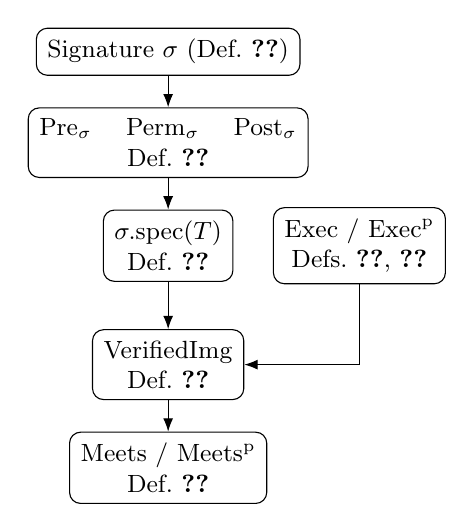
\begin{tikzpicture}[>=Latex,node distance=4mm,b/.style={draw,rounded corners,align=center,font=\small,inner sep=4pt}]
\node[b] (sig) {Signature $\sigma$ (Def.~\ref{def:sig})};
\node[b,below=of sig] (interp) {$\Pre_\sigma$ \quad $\Perm_\sigma$ \quad $\Post_\sigma$\\Def.~\ref{def:prepost}};
\node[b,below=of interp] (spec) {$\sigma.\mathrm{spec}(T)$\\Def.~\ref{def:meets}};
\node[b,right=5mm of spec] (exec) {$\Exec$ / $\Exec^{\mathrm p}$\\Defs.~\ref{def:exec}, \ref{def:execp}};
\node[b,below=6mm of spec] (vi) {$\VI$\\Def.~\ref{def:vi}};
\node[b,below=of vi] (meets) {$\Meets$ / $\MeetsP$\\Def.~\ref{def:meets}};
\draw[->] (sig)--(interp);
\draw[->] (interp)--(spec);
\draw[->] (spec)--(vi);
\draw[->] (exec.south) |- (vi.east);
\draw[->] (vi)--(meets);
\end{tikzpicture}
\caption{A signature is interpreted as concrete preconditions, permissions and postconditions (Definition~\ref{def:prepost}). The interpretation and execution semantics together determine the proposition that the checker must establish. The partial variant uses partial execution in place of total execution in the same construction.}
\Description{A dependency graph connecting signatures to the semantic correctness judgment.}
\end{figure}


$\Meets$ mentions no checker. It says of the code at $e$ in image $c$, with code region $D$: from every entry satisfying the precondition, every execution stays in $D$ until it returns or the process exits, never gets stuck, touches only the bytes of the signature's capabilities and its own stack, terminates, and returns with the preserved registers and the postcondition. The same definition is the target of the checker and of a hand proof of an unsafe function. It can also be used as an explicit hypothesis for an assumed contract. A total meaning implies the partial one (\lean{Meets.toP}).

\begin{example}[Signature of \code{sum}]\label{ex:sig}
In Fig.~\ref{fig:sum}, $X_{\mathrm{in}}=\{\rho,n\}$, $\Gamma_{\mathrm{in}}=\{a_0\mapsto\rho,\ a_1\mapsto n\}$, $\mathcal{B}=\{\top\Rightarrow\bytes{\rho}{8n}{ro}\}$ with no fields, $\mathcal{T}=\mathcal{G}=\emptyset$, $\psi_{\mathrm{pre}}=8\mid\rho$, $X_{\mathrm{out}}=\{r\}$, $\Gamma_{\mathrm{out}}=\{a_0\mapsto r\}$, $\psi_{\mathrm{post}}=\top$, $K=0$.
\end{example}

\begin{example}[Meaning of \code{sum}]\label{ex:meets}
$\Pre$ requires $\un{s.R(a_0)}\equiv\ev{\rho}{\iota}\pmod B$, $\un{s.R(a_1)}\equiv\ev{n}{\iota}\pmod B$, $8\mid\rho$, $0\le\rho$, $0\le 8n$, $\rho+8n\le B$. $\Perm$ makes $[\rho,\rho+8n)$ readable and nothing writable ($K=0$). $\Meets$ for \code{sum} therefore states that every execution reads only $[\rho,\rho+8n)$, writes no memory, terminates, and returns to $\mathit{ra}$ with the preserved registers intact.
\end{example}

%======================================================================
\section{Typing rules}\label{sec:rules}
A function is checked against a \emph{record} $H$ that assigns a state type to each instruction index (Section~\ref{sec:checker}). A rule takes the type $\tau=H(k)$ before the instruction at $k$ to a type $\tau'$ for each successor $k'$, written $\tau\triangleright_i\tau'$; the checker then requires the edge condition $\mathrm{edge}(k,\tau',k')$ of Definition~\ref{def:edge}. Fresh variables are taken above every variable of $\tau$. We write $\tau[r\mapsto e]$ for $\tau$ with $\Gamma(r)=e$ (writes to $x_0$ are ignored), and $\tau\,{+}\,\psi$ for $\tau$ with $\psi$ added to $\Psi$.

\subsection{Arithmetic}
\begin{mathpar}
\inferrule[Addi]{\Gamma(r_s)=e}{\tau\triangleright_{\mathtt{addi}\ r_d,r_s,c}\tau[r_d\mapsto e+c]}
\and
\inferrule[Add]{\Gamma(r_1)=e_1 \\ \Gamma(r_2)=e_2}{\tau\triangleright_{\mathtt{add}\ r_d,r_1,r_2}\tau[r_d\mapsto e_1+e_2]}
\and
\inferrule[Slli]{\Gamma(r_s)=e}{\tau\triangleright_{\mathtt{slli}\ r_d,r_s,h}\tau[r_d\mapsto 2^h e]}
\and
\inferrule[Fresh]{x\ \text{fresh}}{\tau\triangleright_{i}\tau[r_d\mapsto x]\,{+}\,(0\le x<B)}
\end{mathpar}
\textsc{Sub}, \textsc{Sh$N$add}, multiplication by a constant, and \code{lui} are exact in the same way. \textsc{Fresh} applies to any instruction that writes $r_d$ and nothing else; it is always sound and is the fallback when no more precise rule applies. Further rules give fresh variables with facts linking them to their operands: \code{andi} with $2^k-1$ ($e=x+2^kj$), with $-2^k$, and with a single bit; \code{srli}, \code{srliw}; \code{minu}, \code{maxu}; comparisons \code{slt}, \code{sltu} as $0/1$ values with $x=1\Leftrightarrow$ the comparison of representatives; bitwise operations on $0/1$ values; \code{xor} followed by a mask as $a\equiv b\pmod{2^k}$; division and remainder by constants; and the 32-bit forms through $x\equiv e\pmod{2^{32}}$, $-2^{31}\le x<2^{31}$ (\lean{Fn.arith}, \lean{Fn.arithExt}). The stack pointer is written only by the frame rules.

\emph{Soundness} (\lean{Fn.arith\_sound}). If $R(r_s)\models_\iota\inttype{e}$, then $R(r_s)+c\models_\iota\inttype{e+c}$ because the type is a congruence modulo $B$ and machine addition is addition modulo $B$; similarly for the other exact rules (\lean{hasInt\_add}, \lean{hasInt\_smul}, \lean{hasInt\_shl}). For a fresh $x$, the valuation is extended by $\iota(x)=\un{R'(r_d)}$, which satisfies $0\le x<B$ and changes no other variable, so all of $\Psi$ still holds.

\subsection{Branches}
\begin{mathpar}
\inferrule[Bltu]{\Gamma(r_1)=e_1 \\ \Gamma(r_2)=e_2}{\tau\triangleright^{\mathrm{taken}}\tau\,{+}\,u(e_1)<u(e_2) \\ \tau\triangleright^{\mathrm{fall}}\tau\,{+}\,u(e_2)\le u(e_1)}
\and
\inferrule[Beq]{\Gamma(r_1)=e_1 \\ \Gamma(r_2)=e_2}{\tau\triangleright^{\mathrm{taken}}\tau\,{+}\,e_1\eqB e_2 \\ \tau\triangleright^{\mathrm{fall}}\tau\,{+}\,\lnot(e_1\eqB e_2)}
\end{mathpar}
\textsc{Blt} uses the signed representatives; \code{bgeu}, \code{bge}, and \code{bne} swap the two sides.

\emph{Soundness} (\lean{Fn.branch\_sound}). $\un{R(r_j)}$ is the unique value in $[0,B)$ congruent to $\ev{e_j}{\iota}$, so it equals the value of $u(e_j)$ under the valuation extended by the representative's fresh variable; \code{bltu} compares exactly these values. \code{beq} compares words, which are equal iff their values are congruent modulo $B$.

\subsection{Memory}
\begin{definition}[Access condition; \lean{Fn.inCap}, \lean{Fn.addr}]\label{def:access}
For $\tau\in\Ty{STy}$, $a\in\Ty{IExpr}$, byte width $w\in\N$, access mode $m_a\in\Ty{Mode}$, and a held byte capability $h$ whose underlying capability is $\psi\Rightarrow\bytes{b}{n}{m}$ with possible fields and heap mark, define
\[
\begin{aligned}
&\mathrm{Covers}(\tau,h,a,w,m_a)\iff{}\\ &h\in\tau.C\land\tau\ent\psi\\
&\land\big(\tau\ent(b\le a\land a+w\le b+n\land w\mid a)\big)\\
&\land(m_a=\mathsf{rw}\Rightarrow m=\mathsf{rw}).
\end{aligned}
\]
The entailment in parentheses treats the three arithmetic conditions as a single conjunction. This predicate has type $\Ty{STy}\times\Ty{HCap}\times\Ty{IExpr}\times\N\times\Ty{Mode}\to\Prop$. For a load or store with base register $r_s$ and immediate offset $\mathit{off}$, the symbolic address is $a=\tau.\Gamma(r_s)+\mathit{off}$. If no held capability covers it, the checker retries with its unsigned representative $u(a)$.
\end{definition}

\begin{mathpar}
\inferrule[Load]{a=\Gamma(r_s)+\mathit{off} \\ \kappa\in C\ \text{covers}\ (a,w) \\ x\ \text{fresh}}{\tau\triangleright_{\mathtt{l}w\ r_d,\mathit{off}(r_s)}\tau[r_d\mapsto x]\,{+}\,\mathrm{range}_w(x)}
\and
\inferrule[LoadField]{a=\Gamma(r_s)+\mathit{off} \\ \kappa=\bytes{b}{n}{m}\{\dots,k{:}\inttype{e'},\dots\}\in C\ \text{covers}\ (a,8) \\ a-b=k}{\tau\triangleright_{\mathtt{ld}\ r_d,\mathit{off}(r_s)}\tau[r_d\mapsto e']}
\and
\inferrule[Store]{a=\Gamma(r_{1})+\mathit{off} \\ \kappa\in C\ \text{covers}\ (a,w)\ \text{with}\ m=\mathsf{rw}}{\tau\triangleright_{\mathtt{s}w\ r_2,\mathit{off}(r_1)}\tau[\kappa\mapsto\kappa\ \text{with fields}\ \mathrm{upd}(\kappa,a,w,\Gamma(r_2))]}
\end{mathpar}
Here $\mathrm{range}_w(x)$ is $0\le x<2^{8w}$ for unsigned loads and $-2^{8w-1}\le x<2^{8w-1}$ for signed ones. $\mathrm{upd}$ keeps a field only if $\tau$ proves it disjoint from $[a,a+w)$, and an 8-byte store at constant offset $k$ replaces field $k$ with the stored register's expression. Accesses to declared stack slots at $\mathit{sp}+j$ copy expressions between $\Gamma$ and $\Phi(j)$.

\emph{Soundness} (\lean{Fn.load\_sound}, \lean{Fn.store\_sound}, \lean{inCap\_sound}). By validity of $\kappa$, $0\le\ev{b}{\iota}$ and $\ev{b}{\iota}+\ev{n}{\iota}\le B$, so the entailed inequalities place $\ev{a}{\iota}$ and $\ev{a}{\iota}+w$ in $[0,B]$: the effective address computed by the machine modulo $B$ equals $\ev{a}{\iota}$, and every byte of the access lies in $\fp(\kappa)$. By the invariant (I7 below), $\fp(\kappa)$ is readable, and writable if $\kappa$ is exclusive, under the function's permission; with $w\mid a$ the step exists (progress). A load changes only $r_d$. A store changes only bytes of $\fp(\kappa)$; by separation (I5) no other held capability's footprint meets them, so their fields and token invariants are unchanged (by locality of token meanings); fields of $\kappa$ itself are kept only when proved disjoint.

\begin{example}[The load of \code{sum}]\label{ex:load}
At $k=2$, $\Gamma(a_0)=\rho+8n-8m$ and $\Psi\ni 8\mid\rho,\ 1\le m\le n$. The access condition for \code{ld a3, 0(a0)} with the borrowed capability is
\[
\begin{aligned}1\le m\le n,\ 8\mid\rho\ \ent\ {}&\rho\le\rho+8n-8m\ \land\ \rho+8n-8m+8\le\rho+8n\\ {}\land{}&8\mid\rho+8n-8m,\end{aligned}
\]
which the certificate checker proves. The capability has no fields, so \code{a3} receives a fresh $x$ with $0\le x<B$.
\end{example}

\subsection{Control flow and subtyping}
\begin{definition}[Subtyping; \lean{STy.sub}]\label{def:subtype}
A substitution is a finite partial map $\theta\in\Ty{Subst}=\Ty{Var}\rightharpoonup\Ty{IExpr}$. It acts on expressions and constraints by replacing bound variables, leaving other variables unchanged. Subtyping has type $\Ty{STy}\times\Ty{Subst}\times\Ty{STy}\to\Prop$. Write $\tau=(\Gamma,\Psi,C,\Phi,d)$ and $\tau'=(\Gamma',\Psi',C',\Phi',d')$. For held capabilities define $\mathrm{Match}_\tau(h,\theta,h')$ to mean that the identities and origins agree and that the following conditions hold. The target guard implies the source guard under $\tau$ after substitution. Byte capabilities must have the same mode and heap mark, provably equal base and length, and every target field must have a matching source field at the same offset with a congruent expression. Token capabilities must have the same token name. With this predicate the subtyping judgment is
\[
\begin{aligned}
\tau\sub{\theta}\tau'\iff{}& (\forall\psi'\in\Psi'.\ \tau\ent\theta\psi')\\
&\land(\forall(r,e')\in\Gamma'.\ \exists e.\ \Gamma(r)=e\land(\tau\ent e\eqB\theta e'))\\
&\land(\forall h'\in C'.\ \exists h\in C.\ \mathrm{Match}_\tau(h,\theta,h'))\\
&\land d=d'\\
&\land(\forall(j,e')\in\Phi'.\ \exists e.\ \Phi(j)=e\land(\tau\ent e\eqB\theta e')).
\end{aligned}
\]
For byte capabilities the matching entailments include $\tau\ent\theta\psi'\Rightarrow\psi$, $\tau\ent b=\theta b'$, and $\tau\ent n=\theta n'$. Matching fields require $\tau\ent e\eqB\theta e'$ at each target offset.
\end{definition}

\paragraph{Example.} If $\Gamma(a_0)=x+8$ and $\Psi$ entails $x=0$, then a target state type requiring $\Gamma'(a_0)=8$ can be reached with the empty substitution, provided its remaining components meet the subtyping conditions. A target that additionally requires an unavailable writable capability cannot be justified by this argument.


Facts, registers, capabilities, and slots of $\tau$ not mentioned in $\tau'$ are dropped. This is weakening.

\begin{definition}[Loops and edges; \lean{Loop}, \lean{Fn.edgeOk}]\label{def:edge}
For a function with $N$ instructions, let $\Ty{Index}_N=\{0,\ldots,N-1\}$. The visiting order $\mathit{pos}$ assigns positions to instruction indices. A loop $L=(h,\ell,V,\mu)$ contains a head and last index, a finite collection of bound variables $V$, and a measure $\mu\in\Ty{IExpr}$. Its type is represented by $\Ty{Index}_N^2\times\List(\Ty{Var})\times\Ty{IExpr}$. Loop intervals in the visiting order must be nested or disjoint. Let $\mathrm{RespectsBindings}(k,k',\theta)$ mean that $\theta$ binds neither parameters nor entry variables of preserved registers, and that it binds no measure variable of a loop containing both endpoints unless the edge is that loop's own back edge.
\[
\begin{aligned}
&\mathrm{BackOk}(k,\hat\tau,k',\theta)\iff{}\\ &\mathit{pos}(k)<\mathit{pos}(k')\\
&\lor\exists L\in\mathcal L.\ k'=L.h\\ &\quad\land\mathit{pos}(k)\le\mathit{pos}(L.\ell)\\
&\quad\land(\mathit{partial}\lor((\hat\tau\ent0\le L.\mu)\\ &\qquad\land(\hat\tau\ent\theta L.\mu<L.\mu))).
\end{aligned}
\]
For ordinary instruction edges the condition is
\[
\begin{aligned}
\mathrm{edge}(k,\hat\tau,k')\iff{}&k'<N\land\exists\theta\in\Ty{Subst}.\ H(k')\text{ is defined}\\
&\land\mathrm{RespectsBindings}(k,k',\theta)\land\hat\tau\sub{\theta}H(k')\\
&\land\mathrm{BackOk}(k,\hat\tau,k',\theta).
\end{aligned}
\]
The distinguished entry edge checks the entry type against the record at index zero without a loop back-edge obligation. The back-edge condition enforces a nonnegative, strictly decreasing measure for total functions, whereas partial functions do not need a decrease proof.
\end{definition}

The checker computes $\theta$ by a heuristic (from registers typed by a bare variable at the target and from equations among the facts); the heuristic is untrusted, since any $\theta$ is re-checked by subtyping.

\begin{example}[The loop of \code{sum}]\label{ex:tau}\label{ex:back}
The record at the head $k=2$ is
\[
\begin{aligned}H(2)=\big(&\{a_0\mapsto\rho+8n-8m,\ a_1\mapsto m\},\ \{8\mid\rho,\ 1\le m\le n\},\\ &\{\bytes{\rho}{8n}{ro}\},\ \emptyset,\ 0\big),\end{aligned}
\]
with the loop $L=(2,6,\{m\},m)$. On the entry edge from $k=1$, $\theta=\{m\mapsto n\}$ and Example~\ref{ex:beq} supplies $1\le n$. On the back edge from \code{bnez} at $k=6$, $\Gamma(a_1)=m-1$, $\Gamma(a_0)=\rho+8n-8m+8$, the branch adds $\lnot(m-1\eqB0)$, and $\theta=\{m\mapsto m-1\}$; the obligations are $1\le m-1\le n$, $0\le m$, and $m-1<m$.
\end{example}

\subsection{Frames}
A function may declare a frame $\mathit{Fr}=(F,\mathit{slots},\mathit{addr})$ with $16\mid F$, $F\le K$, 8-byte save slots, and address-taken ranges, pairwise disjoint inside $[0,F)$.
\begin{mathpar}
\inferrule[Push]{d=0 \\ \Gamma(\mathit{sp})=e \\ \tau\ent F\le e}{\tau\triangleright_{\mathtt{addi}\ \mathit{sp},\mathit{sp},-F}\tau'}
\and
\inferrule[Pop]{d=F \\ \Gamma(\mathit{sp})=e \\ \text{frame ranges held}}{\tau\triangleright_{\mathtt{addi}\ \mathit{sp},\mathit{sp},F}\tau''}
\end{mathpar}
where $\tau'$ sets $\mathit{sp}\mapsto e-F$ and $d=F$ and adds a held $\bytes{e-F+o}{l}{rw}$ for each address-taken range $(o,l)$, and $\tau''$ sets $\mathit{sp}\mapsto e+F$, $d=0$, $\Phi=\emptyset$, and removes the frame's capabilities, each of which must be held exactly, as \textsf{rw}. The frame's capabilities must be returned at the instruction that raises $\mathit{sp}$, not only at the return, because a call after the epilogue would otherwise run with its stack over a capability still held (\lean{Sound/Frame*.lean}).

\subsection{Calls, system calls, and returns}\label{sec:calls}
A call to a callee $g$ with signature $\sigma_g$ at a known address (\code{jal ra}, or the compiler's pair \code{auipc t}; \code{jalr ra, lo(t)}, where \code{auipc} receives its exact value because the checked image fixes every address) checks, under an instantiation $\theta$ of $X_{\mathrm{in}}(\sigma_g)$ taken from the argument registers:
\begin{mathpar}
\inferrule[Call]{\forall(r,e)\in\Gamma_{\mathrm{in}}^g.\ \tau\ent\Gamma(r)\eqB\theta e \\ \tau\ent\theta\psi^g_{\mathrm{pre}} \\ d+K_g\le K \\
\text{each clause of }\sigma_g\text{ lent from a held capability} \\ \text{\textsf{rw} loans pairwise disjoint}}
{\tau\triangleright\mathrm{afterCall}(\tau,\sigma_g,\theta)}
\end{mathpar}
A \textsf{borrow} or \textsf{take} clause $\bytes{b'}{n'}{m'}$ is lent from a held $\bytes{b}{n}{m}$ with $\tau\ent b\le\theta b'\land\theta b'+\theta n'\le b+n\land0\le\theta n'$, with $m=\mathsf{rw}$ if $m'=\mathsf{rw}$, a whole held \textsf{heap} unit for a \textsf{heap} clause, and fields of the clause present in the held capability; a take clause needs an exclusive capability that did not come from one of the caller's own borrows, and every borrow of the caller must still be held over its whole range at the call. A token clause is lent from the unique held capability of that name. $\mathrm{afterCall}$ keeps preserved registers and slots, gives the $\Gamma_{\mathrm{out}}^g$ registers their types with $X_{\mathrm{out}}^g$ renamed to fresh variables, makes every other caller-saved register a fresh word, adds $\theta\psi^g_{\mathrm{post}}$, removes capabilities lent to take clauses, forgets the fields of capabilities lent \textsf{rw}, and adds the given capabilities.

\code{ecall} requires $a_7$ to be a known constant. For \code{exit} the run ends. For \code{write} and \code{read} of $[b,b+n)$ it requires $0\le n<B$ and a held capability covering the buffer (\textsf{rw} for \code{read}); afterwards $a_0$ is a fresh $x$ with
\[
\begin{aligned}&(-4095\le x\le-1)\ \lor{}\\ &(0\le x\le n\ \land\ x\le\mathtt{0x7ffff000}\ \land\ (\mathtt{write}\land n\ge1\Rightarrow x\ge1)),\end{aligned}
\]
the relation of \lean{Env.lean}, and \code{read} forgets the fields of the capability it wrote into (\lean{Fn.ecallOk}).

\begin{definition}[Return; \lean{Fn.retOkOn}]\label{def:ret}
Fix the function description and signature. The predicate $\mathrm{RetOk}(\tau)$ holds when a substitution $\theta$ for output variables satisfies the following conditions. Write $\mathcal R_{\mathrm{ret}}=\mathcal R_{\mathrm{save}}\cup\{\mathit{ra}\}$.
\[
\begin{aligned}
&\mathrm{RetOk}(\tau)\iff\exists\theta.\\ &\mathrm{dom}(\theta)\subseteq X_{\mathrm{out}}\\
&\land(\forall r\in\mathcal R_{\mathrm{ret}}.\ \tau\ent\Gamma(r)\eqB v_r)\\
&\land(\tau\sub{\theta}(\Gamma_{\mathrm{out}},\{\psi_{\mathrm{post}}\}))\\
&\land\mathrm{BorrowReturn}(\tau,\theta)\\
&\land\big(\mathrm{Transfers}(\sigma)\Rightarrow(d=0\\ &\qquad\land\mathrm{GiveMatch}(\tau,\theta))\big).
\end{aligned}
\]
The shorthand subtyping judgment in the third line checks the output register types and postcondition. The predicate $\mathrm{BorrowReturn}$ requires every borrow clause $i$ to be matched by a held capability of origin $i$ that is a subtype of the exit form. The predicate $\mathrm{Transfers}$ holds when the signature gives capabilities or borrows tokens. The predicate $\mathrm{GiveMatch}$ requires each given capability to be matched by a distinct held exclusive capability that is not returned for a borrow. These conditions are checked for the instruction \code{jalr x0,0(ra)}.
\end{definition}

\paragraph{Example.} If the entry return address is represented by $v_{ra}$ but the type of $ra$ at a return is an unconstrained fresh variable, the return-address congruence cannot be established. The checker therefore rejects the return unless additional facts establish that it restores the original value.


A tail call (\code{auipc t1}; \code{jalr x0}) is a call followed by the return condition of the caller, at depth $0$ with $\mathit{ra}$ the entry's.

%======================================================================
\section{The checker}\label{sec:checker}
\begin{definition}[Function description; \lean{Fn}]\label{def:fn}
A function description $f\in\Ty{Fn}$ is the tuple
\[f=(\sigma,e,N,\mathit{rv},\mathcal L,H,\mathit{Fr},\mathit{pos},\mathit{callees}).\]
Its components have the following mathematical types.
\[
\begin{aligned}
\sigma&\in\Ty{Sig},&e&\in\W,&N&\in\N,\\
\mathit{rv}&:\mathcal R_{\mathrm{ret}}\to\Ty{Var},&\mathcal L&\in\List(\Ty{Loop}),\\
H&:\Ty{Index}_N\rightharpoonup\Ty{STy},&\mathit{Fr}&\in\Opt(\Ty{Frame}),\\
\mathit{pos}&:\Ty{Index}_N\to\Ty{Index}_N,&\mathit{callees}&\in\List(\W\times\Ty{Sig}).
\end{aligned}
\]
The frame type describes a size, save slots, and address-taken ranges as in Section~\ref{sec:rules}. The order is subject to the structural checks below. We write $v_r=\mathit{rv}(r)$ and $pc_k=e+4k$, with word arithmetic for the latter. The record $H$ provides a candidate state type at each annotated instruction, rather than a proof that the state type is correct.
\end{definition}

The signature states the claim, whereas the remaining fields of $f$ are supplied by an untrusted tool and checked.

\begin{definition}[Entry type; \lean{Fn.initTy}]\label{def:initty}
The function $\tau_0:\Ty{Fn}\to\Ty{STy}$ produces the initial type. Its register map includes the signature's entry types and the symbolic entry variables for preserved registers and the return address. Its remaining components are
\[
\begin{aligned}
\tau_0(f).\Psi&=[\psi_{\mathrm{pre}},\ 0\le v_{\mathit{sp}},\ v_{\mathit{sp}}<B,\ 16\mid v_{\mathit{sp}},\ K\le v_{\mathit{sp}}],\\
\tau_0(f).C&=\mathrm{EnumerateHeld}(C_{\mathrm{in}}(\sigma)),\\
\tau_0(f).\Phi&=\emptyset,\qquad\tau_0(f).d=0.
\end{aligned}
\]
Here $\mathrm{EnumerateHeld}$ assigns the entry clause origins $0,1,\ldots$ together with distinct identities. The initial type describes the state before the function allocates its own frame.
\end{definition}
\paragraph{Example.} For the running function, the initial types include $a_0\mapsto\rho$ and $a_1\mapsto n$, while the input capability describes the array and the stack depth is zero. The entry edge must establish the first record type from these facts.

\begin{definition}[Checker; \lean{Fn.check}]\label{def:check}
The executable checker has type $\chk:\Ty{Fn}\times\Ty{Code}\to\Ty{Bool}$. We use $\mathrm{StructOk}:\Ty{Fn}\to\Prop$ for the structural conditions and $\mathrm{InstrOk}:\Ty{Fn}\times\Ty{Code}\times\N\to\Prop$ for the local instruction checks. Its acceptance condition is
\[
\begin{aligned}
\chk(f,c)=\mathit{true}\iff{}&\mathrm{StructOk}(f)\land\mathrm{edge}(\mathrm{entry},\tau_0(f),0)\\
&\land\forall k<N.\ \mathrm{InstrOk}(f,c,k).
\end{aligned}
\]
The structural conditions check the nesting of loops in the visiting order, freshness of measure and bound variables, frame geometry, scope of signature variables, distinct entry capability identities, and compatibility of total and partial callees. Define $\mathrm{RuleOk}(f,k,i,\tau)$ to mean that the rule for the decoded instruction accepts the type and all its successor obligations. Then
\[
\begin{aligned}
\mathrm{InstrOk}(f,c,k)\iff{}\\ & H(k)\text{ is undefined}\\
&\lor\exists i,\tau.\ H(k)=\tau\land c.\mathit{instr}(pc_k)=i\\ &\quad\land\mathrm{RuleOk}(f,k,i,\tau).
\end{aligned}
\]
An unannotated index can be skipped because every accepted incoming edge requires a target type. A return or exit is checked by its terminal rule instead of requiring an ordinary successor annotation.
\end{definition}

\paragraph{Example.} For the running function the record at index 2 asserts that the address register is $\rho+8n-8m$ and that $1\le m\le n$. The checker does not trust this assertion. It establishes the entry edge and the loop back edge using subtyping, then checks the load against the capability and the loop measure against the decrease condition.


The checker runs on the decoded image, so the instructions checked are the instructions executed by the permitted-step semantics. It is an executable Lean function, evaluated by the kernel with \code{decide}.

%======================================================================
\section{The invariant}\label{sec:inv}
\begin{definition}[Invariant; \lean{Inv}]\label{def:inv}
Fix $f$, $T$, an entry state $s_0$, entry valuation $\iota_0$, and entry footprints $F_0$. Let $P=\Perm_\sigma(\iota_0,F_0,s_0)$ and $S=S_K(s_0)$. These are fixed parameters of the invariant. The remaining arguments have type
\[\Inv:\Ty{STy}\times\Ty{State}\times\Ty{Val}\times\Ty{TokenFootprints}\to\Prop.\]
For readability, let $C^*=\mathrm{map}(h\mapsto h.cap,\tau.C)$ denote the underlying capability list, let $A_d$ denote the address-taken ranges of the current frame, and let $\mathrm{Fixed}$ denote signature parameters and entry variables. The invariant is the conjunction $\Inv(\tau,s,\iota,F)\iff\bigwedge_{j=1}^8 I_j$ with the following components.
\begin{align*}
I_1\iff{}&\iota\models\tau.\Psi\land(\forall x\in\mathrm{Fixed}.\ \iota(x)=\iota_0(x)),\\
I_2\iff{}&\mathrm{RegOk}(\tau.\Gamma,\iota,s)\\ &\quad\land s.R(\mathit{sp})=s_0.R(\mathit{sp})-\tau.d\\ &\quad\land s.X=\mathrm{none},\\
I_3\iff{}&\forall(j,e)\in\tau.\Phi.\ \mathrm{SlotOk}(f,\tau.d,j,s_0)\\
&\quad\land\mathrm{load}_{64}(s.M,s.R(\mathit{sp})+j)\models_\iota\inttype{e},\\
I_4\iff{}&\forall h\in\tau.C.\ \Valid_{T,\iota,F}(s.M,h.cap),\\
I_5\iff{}&\Sep_{\iota,F}(C^*)\land\mathrm{DistinctIds}(\tau.C),\\
I_6\iff{}&\forall h\in\tau.C.\ \fp_{\iota,F}(h.cap)\cap S\subseteq A_d,\\
I_7\iff{}&S\subseteq A(P.wr)\land\forall h\in\tau.C.\\
&\quad\fp_{\iota,F}(h.cap)\subseteq A(P.rd)\cup A(P.wr)\\
&\quad\land(\mathrm{exclusive}(h.cap)\Rightarrow\fp_{\iota,F}(h.cap)\subseteq A(P.wr)),\\
I_8\iff{}&16\mid\un{s_0.R(\mathit{sp})}\land K\le\un{s_0.R(\mathit{sp})}\\ &\quad\land(\tau.d=0\lor\tau.d=\mathit{frameSize}).
\end{align*}
The predicate $\mathrm{SlotOk}$ requires a declared slot of the frame at depth $d$ lying in the stack region outside the address-taken ranges. The frame size is taken from the function description. All footprint sets in these formulas are evaluated using the current valuation and token footprints, but the permission $P$ remains fixed at entry.
\end{definition}

\paragraph{Example.} If the invariant holds at the loop head in the running example, $I_2$ identifies the actual address in $a_0$ with $\rho+8n-8m$ modulo $B$. By $I_4$, the array capability is valid, so its interval does not wrap. By $I_1$ and entailment soundness, the access bounds proven from the type hold under the actual valuation. Finally, $I_7$ places the footprint inside the concrete permission. Together these facts establish that the next aligned load has a permitted successor, and its result can be tracked by a fresh logical variable.
\begin{figure*}[t]
\centering
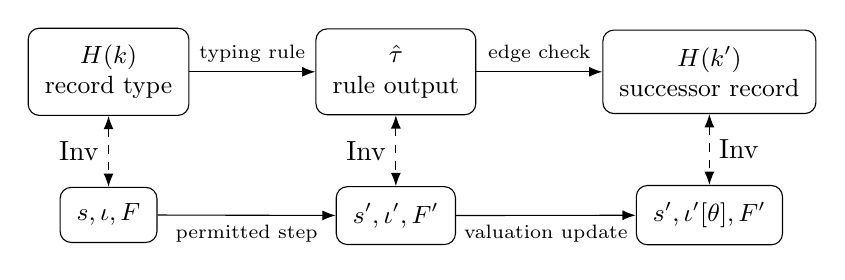
\begin{tikzpicture}[>=Latex,node distance=9mm and 16mm,b/.style={draw,rounded corners,align=center,font=\small,inner sep=6pt}]
\node[b] (t) {$H(k)$\\record type};
\node[b,right=of t] (hat) {$\hat\tau$\\rule output};
\node[b,right=of hat] (next) {$H(k')$\\successor record};
\node[b,below=of t] (s) {$s,\iota,F$};
\node[b,below=of hat] (sp) {$s',\iota',F'$};
\node[b,below=of next] (sn) {$s',\iota'[\theta],F'$};
\draw[->] (t)--node[above,font=\scriptsize]{typing rule}(hat); \draw[->] (hat)--node[above,font=\scriptsize]{edge check}(next);
\draw[->] (s)--node[below,font=\scriptsize]{permitted step}(sp); \draw[->] (sp)--node[below,font=\scriptsize]{valuation update}(sn);
\draw[<->,dashed] (t)--node[left]{$\Inv$}(s); \draw[<->,dashed] (hat)--node[left]{$\Inv$}(sp); \draw[<->,dashed] (next)--node[right]{$\Inv$}(sn);
\end{tikzpicture}
\caption{Local soundness connects a checked instruction rule to a concrete permitted transition. The edge check then establishes the successor record type under a substituted valuation. For total functions the rank decreases along accepted edges. Calls use a corresponding multi-step argument.}
\Description{A commuting-style diagram of the invariant, instruction rule, and edge check.}
\end{figure*}


I5 removes aliasing; I6 keeps save slots and the callees' stack out of every capability; I7 gives progress at accesses and, at the return, the pool condition. Table~\ref{tab:inv} lists what each part connects.

\begin{table}[t]
\caption{Parts of the invariant and the obligations they discharge.}
\label{tab:inv}
\centering\small
\begin{tabular}{@{}lll@{}}
\toprule
Part & Relates & Used for\\
\midrule
I1 & $\iota$ and $\Psi$ & entailments are true facts\\
I2, I3 & registers, slots, and $\Gamma,\Phi$ & values of operands\\
I4 & memory and $C$ & address bounds, field values\\
I5 & footprints of $C$ & stores change no other capability\\
I6 & $C$ and the stack & slots and callee stacks unaffected\\
I7 & $C$ and $P$ & progress; pool at return\\
I8 & frame geometry & frame rules, call stack bound\\
\bottomrule
\end{tabular}
\end{table}

%======================================================================
\section{Soundness}\label{sec:soundness}
Fix $f$ with $\chk(f,c)$, an entry state $s_0$ with $\Entry_D(e,s_0)$ and $\Pre_\sigma(T,\iota_0,F_0,s_0)$, and $P=\Perm_\sigma(\iota_0,F_0,s_0)$. The entry valuation $\iota_0^f$ extends $\iota_0$ with $v_r\mapsto\un{R_0(r)}$ for the preserved registers and the remaining entry variables (\lean{Fn.entryVal}). The lemmas below are stated for one function; calls are treated in Section~\ref{sec:compose}.

\begin{lem}[Initialization; \lean{Fn.entry\_inv}]\label{lem:init}
$\Inv(\tau_0(f),s_0,\iota_0^f,F_0)$.
\end{lem}
\begin{proof}[Proof sketch]
I1 from $\Pre$ and the definition of $\iota_0^f$; I2 by construction of $\iota_0^f$; I4, I5 from validity and separation in $\Pre$; I6 because no entry footprint meets the stack region; I7 because $P$ is built from the entry footprints and the stack region; I8 from $\Entry$ and $K\le\un{R(\mathit{sp})}$.
\end{proof}

\begin{lem}[Weakening; \lean{Inv.sub}]\label{lem:weak}
If $\Inv(\tau,s,\iota,F)$, $\tau\sub{\theta}\tau'$, and $\theta$ binds no protected variable, then $\Inv(\tau',s,\iota[\theta],F)$, where $\iota[\theta](y)=\ev{\theta y}{\iota}$ for $y$ bound by $\theta$ and $\iota(y)$ otherwise.
\end{lem}
\begin{proof}[Proof sketch]
Each condition of Definition~\ref{def:subtype} is an entailment from $\mathrm{hyps}(\tau)$, true under $\iota$ by I1, I4, and Theorem~\ref{thm:entail}; evaluating $\theta e'$ under $\iota$ equals evaluating $e'$ under $\iota[\theta]$. Capabilities of $\tau'$ correspond to capabilities of $\tau$ with equal footprints, so I4--I7 transfer, and dropped capabilities only weaken I5.
\end{proof}

\begin{lem}[Progress and preservation; \lean{Fn.runStep}]\label{lem:step}
If $\Inv(H(k),s,\iota,F)$ and $s.pc=\mathit{pc}_k$, then $s$ has a $\Step(c,P)$ successor (or, for a call, the callee's execution is safe and ends), and every successor $s'$, or every state in which the callee returns, satisfies $\Inv(\hat\tau,s',\iota',F')$ for the rule's output $\hat\tau$ towards $k'$ and an extension $\iota'$ of $\iota$ that agrees with it below the fresh variables; or $s'$ is final and satisfies $\Done$.
\end{lem}
\begin{proof}[Proof sketch]
The proof proceeds by cases on the decoded instruction and applies the corresponding lemma. The cases are covered by \lean{Fn.arith\_sound} and \lean{Fn.arithExt\_sound} (arithmetic), \lean{Fn.branch\_sound}, \lean{Fn.load\_sound} and \lean{Fn.store\_sound} (Section~\ref{sec:rules}), the slot and frame lemmas (\lean{Fn.slotLoad\_sound}, \lean{Fn.slotStore\_sound}, \lean{Fn.framePop\_sound}), \lean{Fn.ecall\_step}, \lean{Fn.call\_step} (Section~\ref{sec:compose}), \lean{Fn.tail\_step}, and the return (Lemma~\ref{lem:ret}). The unit frame of $\Post$ is carried along the run by an auxiliary invariant over the $\mathsf{Heap}$ footprint relative to the entry (\lean{Fn.UnitFrame}).
\end{proof}

\begin{lem}[Edges; \lean{Fn.edgeOk\_sound}]\label{lem:edge}
If $\mathrm{edge}(k,\hat\tau,k')$ holds with $\theta$ and $\Inv(\hat\tau,s,\iota,F)$, then $k'<N$, $\Inv(H(k'),s,\iota[\theta],F)$, and, for a non-partial function, $\rank(k',\iota[\theta])<\rank(k,\iota)$.
\end{lem}

The ranking function (\lean{Fn.rank}) assigns to each loop $L$, in order of heads, the pair $(2,0)$ before $L$, $(1,\ev{\mu_L}{\iota}+1)$ inside $L$, and $(0,0)$ after it, followed by $(0,N-\mathit{pos}(k))$; pairs and lists are ordered lexicographically, which is well-founded (\lean{LexN.wf}). A forward edge leaves the components of loops containing both ends unchanged, because $\theta$ cannot rebind their measure variables, and decreases the last component (\lean{rank\_fwd}); a back edge to the head of $L$ decreases $L$'s component by the measure condition and leaves the components of enclosing loops unchanged (\lean{rank\_back}). This replaces an argument about the outermost loop traversed infinitely often.

\begin{lem}[Return; \lean{Fn.retOk\_sound}]\label{lem:ret}
If the return condition holds at $\tau$ and $\Inv(\tau,s,\iota,F)$, then the step of \code{jalr x0, 0(ra)} reaches $R_0(\mathit{ra})$ with the preserved registers of $s_0$ and $\Post_\sigma(T,\iota_0,F_0,s_0,s')$.
\end{lem}
\begin{proof}[Proof sketch]
The registers follow from I2 and the congruences, which are equalities of words. $\Post$'s valuation is $\iota[\theta]$, which agrees with $\iota_0$ outside $X_{\mathrm{out}}$ by I1. The exit capabilities are held (validity by I4, separation by I5). A given capability or borrowed token is held exclusively at depth $0$ and is not the capability of any borrow; by I6 at depth $0$ it misses the stack, by I7 it lies in the writable entry footprints, and by I5 it misses every returned borrow; what remains of the writable entry footprints is the pool.
\end{proof}

\begin{claim}[Soundness of the checker; \lean{Fn.check\_sound}]\label{thm:check}
Let $\chk(f,c)$ hold, $f$ not partial, $D$ contain $\mathit{pc}_k$ for every $k<N$, and every callee $(a,\sigma_g)$ of $f$ satisfy $4\mid a$ and $\Meets(c,D_g,a,T,\sigma_g)$ for some $D_g\subseteq D$ disjoint from $f$'s instructions. Then
\[
\boxed{\;\Meets(c,D,e,T,\sigma).\;}
\]
\end{claim}
\begin{proof}[Proof sketch]
Given an entry state, Lemma~\ref{lem:init} gives $\Inv$ at $\tau_0(f)$ and Lemma~\ref{lem:edge} carries it to $H(0)$. \lean{Fn.run} proves, by well-founded induction on $(k,\iota)$ ordered by $\rank$, that from every state at $\mathit{pc}_k$ satisfying $\Inv(H(k),\dots)$ the execution satisfies $\Exec(c,P,D,\Done)$: Lemma~\ref{lem:step} gives a step and $\Inv$ at the output type, Lemma~\ref{lem:edge} carries it to $H(k')$ with a smaller rank, and the induction hypothesis applies; a return or exit is final by Lemma~\ref{lem:ret}. The token footprints may change along the run (calls replace a lent token's footprint), so the induction quantifies over them.
\end{proof}

For a function without callees this is \lean{Fn.check\_sound\_leaf}, with $D$ the function's own instructions.

\begin{claim}[Partial soundness; \lean{Fn.check\_soundP}]\label{thm:checkp}
Under the hypotheses of Theorem~\ref{thm:check} without the restriction to non-partial functions, with callees satisfying $\MeetsP$, $\chk(f,c)$ implies $\MeetsP(c,D,e,T,\sigma)$.
\end{claim}
The proof replaces the rank by the step index of $\Exec^{\mathrm p}$ (\lean{Fn.runP}); a partial function needs no measures, and a total function may call no partial one.

\begin{example}[\code{sum}, end to end]\label{ex:final}
For the nine words of \code{sum} as assembled by clang and the record of Example~\ref{ex:tau}, the kernel evaluates $\chk(f_{\mathtt{sum}},c)=\mathit{true}$, and Theorem~\ref{thm:check} yields the Lean theorem \lean{sum\_meets}: $\Meets(c,[(e,36)],e,T,\sigma_{\mathtt{sum}})$ for every $T$, the statement of Example~\ref{ex:meets}. It does not say that the returned value is the sum, which is a functional property for a separate proof that can now assume memory safety, the frame, and termination. Six faulty variants (a buffer one word short, no alignment fact, a non-decreasing measure, a false fact in the record, an offset reading past the buffer, a return through \code{a1}) are rejected.
\end{example}

%======================================================================
\section{Calls and programs}\label{sec:compose}
\begin{lem}[Calls; \lean{Fn.callee\_pre}, \lean{Fn.afterCall\_inv}, \lean{Fn.call\_step}]\label{lem:call}
If the call rule accepts a call of $g$ at $k$ and $\Inv(H(k),s,\iota,F)$, then the state after the jump satisfies $\Entry_{D_g}$ and $\Pre_{\sigma_g}$ under $\iota[\theta]$, and $\Perm_{\sigma_g}\le P$; and every state in which the callee returns, satisfying $\Done_g$ and the frame property, satisfies $\Inv(\mathrm{afterCall}(\tau,\sigma_g,\theta),s',\iota',F')$.
\end{lem}
\begin{proof}[Proof sketch]
The callee's clauses lie inside held footprints, so they are valid with non-negative lengths (I4 and the lending condition) and readable or writable under $P$ (I7); with the byte-wise judgment this gives $\Perm_{\sigma_g}\le P$ even when a lent range spans several regions of $P$. Separation of the clauses follows from I5 for different holders and from the disjointness check for loans from one holder. The callee's stack lies below the caller's frame inside $S_K(s_0)$ by $d+K_g\le K$ and misses every footprint by I6. After the return, memory has changed only in the callee's writable bytes, which comprise lent \textsf{rw} ranges, taken exclusive ranges, lent tokens, and its stack. Capabilities kept by the caller lose only the fields that a \textsf{rw} loan may have changed; given capabilities lie in the callee's pool, which the caller lent and no longer holds, so separation is preserved; a \textsf{heap} block the caller kept misses the callee's pool and stack, so by the callee's unit frame it is still a unit. \lean{VerifiedImg.call} composes the callee's execution with the caller's.
\end{proof}

\begin{definition}[Programs; \lean{Prog.check}]\label{def:prog}
A program environment has type $\Ty{Env}=\List(\W\times\Ty{Sig}\times\Ty{Domain})$. We use $\mathcal E$ for this environment to distinguish it from the event trace of a machine state. Program checking is a Boolean function on a code image, an environment, and a list of function descriptions.
\[
\begin{aligned}
&\mathrm{Prog.check}(c,\mathcal E,[])=\mathit{true},\\
&\mathrm{Prog.check}(c,\mathcal E,f::fs)=\mathit{true}\iff{}\\ &\quad\chk(f,c)=\mathit{true}\land\neg f.\sigma.\mathit{partial}\\
&\land\mathrm{CalleesOk}(f,\mathcal E)\\
&\land\mathrm{Prog.check}(c,(f.e,f.\sigma,D_f)::\mathcal E,fs)=\mathit{true}.
\end{aligned}
\]
The predicate $\mathrm{CalleesOk}$ requires every callee address and signature to occur in $\mathcal E$, with aligned entry address and domain disjoint from the instructions of $f$. The domain $D_f$ comprises the instructions of $f$ and the domains of its callees. The list constructor $::$ prepends one element. In particular a function may call an external function or a function checked earlier in the list, but cannot call a later function recursively.
\end{definition}

\paragraph{Example.} If $g$ is a leaf function and $f$ calls $g$, the list $[g,f]$ permits the checker to add the verified signature of $g$ to the environment before checking $f$. With an initially empty environment, the reverse order fails the callee lookup.


\begin{claim}[Programs; \lean{Prog.check\_sound}]\label{thm:prog}
If $\mathrm{Prog.check}(c,\mathcal E,f_1\dots f_m)$ and every $(a,\sigma,D)\in\mathcal E$ satisfies $\Meets(c,D,a,T,\sigma)$, then every entry of the extended environment does; in particular each $f_i$ meets its signature on its domain. For $\mathcal E=\emptyset$ the conclusion is unconditional (\lean{Prog.check\_sound\_closed}).
\end{claim}
\begin{proof}[Proof sketch]
Induction on the list, applying Theorem~\ref{thm:check} to each function with its callees taken from the environment built so far. The order excludes recursion because a function may call only functions earlier in the list or in $\mathcal E$.
\end{proof}

%======================================================================
\section{Safe and unsafe functions}\label{sec:unsafe}
The environment $\mathcal E$ of Theorem~\ref{thm:prog} is where unsafe code enters. An unsafe function has a signature and a body that is not checked; its entry in $\mathcal E$ is a hypothesis $\Meets(c,D,a,T,\sigma)$, the same proposition the checker establishes for safe functions. Table~\ref{tab:evidence} lists the kinds of evidence for $\sem{\sigma}$. Token meanings are where an unsafe module states what its private memory holds; locality (Definition~\ref{def:tok}) is the obligation that lets safe code carry a token across stores without knowing its meaning.

\begin{table}[t]
\caption{Evidence for $\sem{\sigma}$. All rows state the same proposition (Definition~\ref{def:meets}).}
\label{tab:evidence}
\centering\small
\begin{tabular}{@{}p{24mm}p{26mm}p{25mm}@{}}
\toprule
Evidence & Status in Lean & Trusted\\
\midrule
Lean checker (safe) & theorem (Thm.~\ref{thm:check}, \ref{thm:prog}) & definitions only\\
Proof by hand (unsafe) & theorem & definitions only\\
Rust checker (safe) & none & the Rust checker\\
Assumed contract & hypothesis in $\mathcal E$ & the contract\\
\bottomrule
\end{tabular}
\end{table}

Code that the machine model cannot execute (compressed or floating-point instructions, other system calls) has no $\Step$ successor, so a hypothesis $\Meets$ about it would be false; such code needs an environment step of its own, which the model does not yet have.

%======================================================================
\section{From the model to the hardware step}\label{sec:hw}
\begin{claim}[Hardware; \lean{VerifiedImg.hw}]\label{thm:hw}
Let $\VI(c,D,e,\mathit{sp})$, $\Entry_D(e,s)$, $\mathit{pre}(a,s)$, memory of $s$ hold the image $c$ (\lean{Code.Loaded}), no writable byte of $\mathit{perm}(a,s)$ lie in the image (\lean{Protected}), and $4\mid c.\mathit{base}$. Then every $\HwStep$-execution from $s$ that is still in $D$ can step, and each of its steps is a $\Step(c,\mathit{perm}(a,s))$ step; every such execution that leaves $D$ or exits satisfies $\Done(a,s)$; and no $\HwStep$-execution stays in $D$ forever.
\end{claim}

Under the callee and domain hypotheses of Theorem~\ref{thm:check}, acceptance establishes $\Meets$. By Definition~\ref{def:meets}, this is precisely $\VI$ for the interpreted signature. When the image is loaded, protected and aligned as required by Theorem~\ref{thm:hw}, this property transfers to the hardware-step model. Consequently, the final guarantee concerns the loaded machine code within the modeled instruction semantics, rather than a proof of agreement with physical hardware.

\subsection{What is trusted}
The interpretation of Theorem~\ref{thm:check} depends on the definitions of the decoder and instruction semantics, the system-call relation, $\Step$, $\Reach$, $\Exec$, $\VI$ (\lean{Isa}, \lean{Machine}, \lean{Env}, \lean{Step}, \lean{Spec}), and the type language and $\sem{\sigma}$ (\lean{Typed/Lang}, \lean{Typed/Sem}, \lean{Typed/SemPartial}) as well as on the Lean kernel. The record, loops, measures, instantiations, and the certificate search are hints, re-checked or checked. Everything uses only \lean{propext}, \lean{Classical.choice}, and \lean{Quot.sound}; no declaration uses \lean{sorry} or \lean{native\_decide}. The remaining trust assumptions and limitations are as follows.
\begin{itemize}
\item The machine model is compared against reference tools by testing rather than by proof. The decoder agrees with \code{llvm-mc} on 230,005 instruction words, and the semantics with QEMU and with the Sail RISC-V model~\cite{sailriscv} on 48 programs each. Signals, threads, other processes, and other system calls are outside the model.
\item Hypotheses in $\mathcal E$ (assumed contracts) and token meanings are trusted as stated.
\item Functions accepted only by the Rust checker (Section~\ref{sec:impl}) rely on that checker; its ledger marks them \emph{checked}, and marks \emph{proved} only programs for which Theorem~\ref{thm:prog} was obtained in Lean.
\end{itemize}

%======================================================================
\section{Implementation}\label{sec:impl}
\begin{table}[t]
\caption{Components at the pinned commit; lines including comments.}
\label{tab:components}
\centering\small
\begin{tabular}{@{}lr@{}}
\toprule
Component & Lines\\
\midrule
Lean machine model, program logic, adequacy & 1,684\\
Lean type language, $\sem{\sigma}$, partial meaning & 460\\
Lean entailment and certificates & 767\\
Lean checker, rules, programs & 1,591\\
Lean soundness (43 files) & 7,354\\
Lean kernel-checked examples & 494\\
Rust checker, ledger, export & 10,471\\
\bottomrule
\end{tabular}
\end{table}

Table~\ref{tab:components} summarizes the development. Two checkers implement the rules. The \emph{Rust checker} reads assembly as compilers emit it, with signatures and annotations in assembler comments, so the same file goes to the assembler; it infers the record by one pass per function, decides entailments with its own Omega-test procedure~\cite{omega} over checked 128-bit integers (overflow or an exhausted budget answers ``not proved''), compares the instructions it checked with the words of the assembled object, links several files into a program, and exports each accepted function's description and record as a Lean module. The \emph{Lean checker} of Section~\ref{sec:checker} takes that export, re-checks it on the linked image, and, when every function of a closed program is accepted, the kernel's evaluation of $\mathrm{Prog.check}$ and Theorem~\ref{thm:prog} give a theorem per function; only then does the ledger record \emph{proved}. Both checkers decide the same rules, and a shared corpus of programs with expected verdicts, including one rejected case per rule, keeps them aligned.

%======================================================================
\section{Evaluation}\label{sec:eval}
\paragraph{Kernel-checked examples.} Besides \code{sum} (Example~\ref{ex:final}), the Lean examples include a function with a stack frame, save slots, and an address-taken buffer (\lean{f\_meets}); a \code{write} system call (\lean{write\_meets}); a \code{read} into a borrowed buffer; and functions reading static data, including a field of a known word. Each has rejected variants: \code{ra} reloaded from outside the frame, a store past an address-taken range, an epilogue returning half the frame, a frame larger than the stack bound, a \code{read} into a read-only buffer, a buffer one byte too short, an unmodeled system call, and a wrong claimed value of a static word.

\paragraph{Corpus.} The shared corpus holds 140 expected verdicts. It includes the design's examples, accepted and rejected cases for every rule (bounds off by one, overlapping writable loans, use after \code{free}, double \code{free}, a missing null check, recursion, an overrun through \code{read}), contracts, and the trial functions below. The Rust checker meets all of them. Checking the 38 accepted functions of an earlier, smaller corpus took 46.9\,ms in total on one core (median 0.4\,ms, maximum 14\,ms with 80 entailment queries).

\paragraph{Unmodified compiler output.} We took 29 functions of musl 1.2.5~\cite{musl} and two allocator contracts, compiled with clang 15.0.7 for \code{rv64im\_zba\_zbb} at \code{-O2} without compressed instructions, linker relaxation, or jump tables, and wrote signatures and loop annotations without changing an instruction; a script checks that each annotated file assembles to the bytes, relocations, and constant pools of the original object. The predicted verdict of each function was fixed before it was compiled. Table~\ref{tab:musl} gives the predictions and both checkers' verdicts.

\begin{table}[t]
\caption{musl 1.2.5 compiled as is: verdict predicted before compiling (P), the Rust checker's verdict (R), and the Lean checker's verdict on the Rust checker's exported record (L; ?: no verdict within the evaluation limits; --: no record, since the Rust checker rejects). A: accepted; R: rejected although a natural safe signature exists; X: the contract (or a callee's) is not expressible; U: needs an unsafe contract; E: external contract (does not compile without atomics). In column L, R means the Lean checker rejects.}
\label{tab:musl}
\centering\small
\begin{tabular}{@{}lccc@{\quad}lccc@{}}
\toprule
Function & P & R & L & Function & P & R & L\\
\midrule
\code{labs} & A & A & A & \code{memmove} & R & A & ?\\
\code{memcmp} & A & A & A & \code{strlen} & X & X & --\\
\code{bcmp} & A & A & R & \code{fwrite} & U & R & --\\
\code{memrchr} & A & A & R & \code{malloc} & U & E & --\\
\code{memchr} & A & R & -- & \code{free} & U & E & --\\
\code{strnlen} & A & A & R & \code{wmemcpy} & A & A & R\\
\code{strncmp} & A & A & R & \code{wmemset} & A & A & R\\
\code{swab} & A & A & A & \code{wmemcmp} & A & A & A\\
\code{bzero} & A & A & R & \code{wmemchr} & A & A & A\\
\code{memset} & R & A & R & \code{stpncpy} & R & A & ?\\
\code{memcpy} & R & A & ? & \code{strncpy} & A & A & R\\
\code{memccpy} & R & A & ? & \code{\_Exit} & A & A & A\\
\code{\_\_towrite} & A & A & A & \code{ffsl} & A & A & R\\
\code{\_\_fwritex} & R & R & -- & \code{div} & A & A & A\\
\code{bsearch} & R & R & -- & \code{a64l} & X & X & --\\
\code{l64a} & R & A & R & & & &\\
\bottomrule
\end{tabular}
\end{table}

The Rust checker accepts 23 of the 29 compiled functions, in 0.1 to 182\,ms each; linked as one program, 22 of them form a closed safe program (\code{strnlen} calls the rejected \code{memchr}). The predictions were made against the initial rule table; the rules that turned predicted rejections into acceptances (bit masks with negative and single-bit constants, $0/1$ comparison results, \code{xor} followed by a mask as a congruence, read-only data, and loops as natural loops of a reducible graph rather than address intervals) are general facts about instructions and control flow, prompted by this code. We identified the causes of the six rejections. They involve two indirect calls through function pointers (\code{\_\_fwritex}, \code{bsearch}), outside the profile; \code{strlen} and \code{a64l} (through \code{strchr}), whose precondition, a NUL byte in readable memory, is not a signature of this language; a non-linear length $\mathit{size}\cdot\mathit{nmemb}$ (\code{fwrite}); and \code{memchr}, where the compiler joins two paths and the aligned word loop is safe only because of a fact about a byte loaded on one of them, which the type language does not keep.

The Lean checker, evaluated on the decoded words of each object with the Rust checker's exported record, accepts 8 of the 23 functions the Rust checker accepts and gives no verdict on 4 (\code{memcpy}, \code{memccpy}, \code{memmove}, \code{stpncpy}, whose records of 79 to 368 queries exceed the evaluation limits); it accepts nothing the Rust checker rejects. Each of its 11 rejections stops at an instruction for which it lacks a rule or an input that the Rust checker has. The missing support concerns compiler call sequences in unlinked objects, implicit read-only data capabilities absent from the export, re-establishing a loop annotation from an equation rather than a register, $0/1$ bitwise operations, and \code{andi} with $-2^k$. These results show incompleteness of the Lean checker relative to the Rust checker rather than disagreements about soundness. Until these gaps are closed, the 15 functions concerned rely on the Rust checker.

One signature records an assumption of the code. \code{memmove} decides that two ranges do not overlap with the unsigned test $s-d-n\le-2n$, which implies disjointness only for $n<2^{63}$; for larger $n$ it passes overlapping ranges to \code{memcpy}. The checker rejected the signature with $n<2^{64}$, and an exhaustive search with $2^6$ in place of $2^{64}$ finds counterexamples only for $n>2^5$. The accepted signature states $n<2^{63}$, which C's bound on object sizes guarantees.

\paragraph{Execution as a test.} Independently of the proofs, every accepted function was run 300 times on an interpreter that enforces the permission of its signature, from random entry states satisfying the signature and with callees simulated by their contracts; no run faulted. The same interpreter faults on seven corpus functions the checker rejects for memory reasons.

%======================================================================
\section{Related work}\label{sec:related}
\emph{Proof-carrying code and typed assembly.} Necula and Lee certified hand-tuned packet filters with safety proofs checked at load time~\cite{pcc96,pcc97}, the precedent for checking a recorded derivation rather than repeating a search. TAL~\cite{tal} types the output of a type-preserving compiler, and DTAL~\cite{dtal} adds linear integer index types; \sys's $\inttype{e}$ follows DTAL, defined modulo $2^{64}$ for a concrete 64-bit machine. Alias types~\cite{aliastypes} separate pointers from the permission to use them, as capabilities do here, and LTAL~\cite{ltal} types memory management with linear types. FunTAL~\cite{funtal} formalizes the boundary between a functional language and typed assembly; \sys's boundary is between checked and unchecked machine code. These systems are proved sound against abstract machines; \sys's soundness is a machine-checked theorem about an instruction-set semantics.

\emph{Isolation.} Software fault isolation~\cite{sfi}, Native Client~\cite{nacl}, and RockSalt~\cite{rocksalt}, which verifies a sandbox checker against an x86 model, confine a whole module. PREVAIL~\cite{prevail} checks eBPF extensions by abstract interpretation, and the Linux verifier's range analysis has been verified~\cite{ebpfrange}. They establish isolation, not per-function contracts with ownership transfer.

\emph{Refinement and ownership types.} Liquid types~\cite{liquid,llliquid} refine values with predicates and infer annotations. RefinedC~\cite{refinedc} and CN~\cite{cn} combine refinement types with separation-logic ownership for C. RustBelt~\cite{rustbelt} gives types a semantic meaning in separation logic~\cite{seplogic} and verifies unsafe libraries against it, the stance \sys\ takes for unsafe contracts, at the level of machine code and without lifetimes, sharing, or concurrency.

\emph{Machine-code verification.} Decompilation into logic~\cite{myreen}, translation validation of seL4~\cite{sel4tv}, and Islaris~\cite{islaris} over Sail models~\cite{sail} prove functional properties of machine code. \sys\ discharges the memory-safety, frame, and termination part of such proofs by type checking, and a hand proof of an unsafe function targets the same $\sem{\sigma}$.

%======================================================================
\section{Conclusion}
\sys\ gives machine code a type system whose judgments mean one proposition, $\sem{\sigma}$, defined over an instruction-set semantics. The checker that decides the judgments is itself defined in Lean and proved to establish $\sem{\sigma}$, so for a function it accepts, memory safety relative to its capabilities, the calling convention, ownership transfer, and termination are kernel-checked theorems about the decoded image, conditional only on the signatures of its callees. Unmodified compiler output of a C library is largely within reach of the language. The remaining limitations include NUL-terminated strings, function pointers, non-linear lengths, and path-dependent facts at joins, which are the next extensions of the type language.

\bibliographystyle{ACM-Reference-Format}
\bibliography{nocompiler-references}

\appendix
\section{Summary of definitions}
\begin{center}\small
\begin{tabular}{@{}p{30mm}p{19mm}p{24mm}@{}}
\toprule
Object & Definition & Lean\\
\midrule
state, image, $\HwStep$ & \ref{def:state}, \ref{def:hwstep} & \lean{State}, \lean{Code}, \lean{HwStep}\\
permission, $\canRead$ & \ref{def:perm} & \lean{Perm}\\
$\Step$ & \ref{def:step} & \lean{Step}\\
$\Reach$, $\Exec$ & \ref{def:exec} & \lean{Reach}, \lean{Exec}\\
partial execution & \ref{def:execp} & \lean{ReachP}, \lean{ExecP}\\
index expr., constraint & \ref{def:index} & \lean{IExpr}, \lean{Constr}\\
$w\models_\iota\inttype{e}$ & \ref{def:hasint} & \lean{HasInt}\\
capability, validity & \ref{def:cap}, \ref{def:valid} & \lean{Cap}, \lean{Cap.valid}\\
token meaning & \ref{def:tok} & \lean{TokDef}\\
separation & \ref{def:sep} & \lean{Separated}\\
state type & \ref{def:sty} & \lean{STy}\\
certificate & \ref{def:cert} & \lean{Cert}, \lean{Query}\\
signature & \ref{def:sig} & \lean{Sig}\\
$\Pre$, $\Perm$, $\Post$ & \ref{def:prepost} & \lean{Sig.spec}\\
$\VI$ & \ref{def:vi} & \lean{VerifiedImg}\\
$\Meets$, $\MeetsP$ & \ref{def:meets} & \lean{Meets}, \lean{MeetsP}\\
subtyping & \ref{def:subtype} & \lean{STy.sub}\\
edge condition & \ref{def:edge} & \lean{Fn.edgeOk}\\
function description & \ref{def:fn} & \lean{Fn}\\
entry type & \ref{def:initty} & \lean{Fn.initTy}\\
checker & \ref{def:check} & \lean{Fn.check}\\
invariant & \ref{def:inv} & \lean{Inv}\\
program check & \ref{def:prog} & \lean{Prog.check}\\
\bottomrule
\end{tabular}
\end{center}
The development rests on the meaning of a state type ($\Inv$, Definition~\ref{def:inv}), local soundness (Lemmas~\ref{lem:weak}--\ref{lem:ret}, which establish invariant preservation and rank decrease along accepted edges for total functions), and global soundness (Theorems~\ref{thm:check} and~\ref{thm:prog}, which establish the signature meaning under their stated hypotheses).
\end{document}
